\section{Wall-function in FVM CFD: Spatial-discretization error and sampling sensitivity}
\label{subsec:comparative:zpg:yplus-sensitivity}

The closure assessment in Section~\ref{sec:comparative:zpg:cross-comparison} determines how accurately a wall function recovers wall loads from a prescribed, ideal, boundary layer state. In CFD, that state is itself part of a discrete solution. Consequently, a change in sampling height can alter both the closure response and the numerical solution of the surrounding boundary layer. This section analysis the behaviour of the wall functions on the LowH\_M3 and M6Tw025 cases, by first examining their accuracy and consistency on a conventional mesh strategy as the wall functions were intended to be used e.g. by Li et al. in \cite{li2025WF}. Subsequently, a novel boundary layer-informed mesh design is introduced to isolate the identified internal-face discretization errors. Finally the, in the previous section identified, closure discrepancies are revisited in the context of the new meshes, by presccribing an ideally fitted closure to isolate out all found error effects, but from the turbulence models.

\subsection{Wall functions on conventional meshes}
\label{subsec:comparative:zpg:conventional-mesh}

The conventional mesh strategy and sampling geometry are introduced in Section~\ref{subsec:wall-functions:sampling-geometry}. The general idea how conventionally meshes for wall-functions are designed is, to increase the first-cell height until the desired \(y^+_1\) is achieved. In these \textit{conventional wall-function mesh} sweeps, increasing the physical first-cell height moves the wall-function sample outward and increases the separation of neighbouring cell centres. Thus, on \textit{conventional wall-function mesh} the sampling location $y_s^+$ coincides with the first-cell location $y_1^+$, while the spacing of internal-face stencils, herin referred to as \(h^+\),  changes with it (see Figure~\ref{fig:WF:exemplaray_y+10_mesh} \(h^+\) change between exemplary \(y^+_1 = 10\) and \(y^+_1 = 30\) meshes). One should keep in mind, that the sample height $y_s^+$ and physical first-cell mesh resolution \(y^+_1\) need not necessarily be identical, but one could also take the second off-wall cell centre as the wall function sampling point. This distinction becomes essential when the two are varied independently below.
\par\medskip

Figure~\ref{fig:WF:mesh} shows a representative conventional M6Tw025 mesh with special attention to the leading edge region. The leading edge requires additional care because the local friction velocity and the boundary layer thickness differ substantially from their downstream values at which the sampling station with the desired \(y^+_1\) is specified. With a constant physical first-cell height, the elevated upstream shear raises $y_1^+$ significantly above its intended value at the comparison station. For coarse meshes it was found, that \(y^+_1\) at the leading edge region even spiked beyond values where the wall-function is applicable and resulted in unphyiscal behaviour which propagates downstream. Figure~\ref{fig:WF:mesh_constant_smooth} illustrates this effect and its reduction by smoothly increasing the first-cell height over the initial $80\,\mathrm{mm}$ of the plate, thus giving a clearer picture of the actual wall-function behaviour.

\begin{figure}[H]
    \centering
    % Figure provenance (WSL; absolute paths):
    %   Figure: /mnt/c/Users/MichaelGnadlinger/OneDrive - Hypersonica/Hypersonica Team - Documents/02 Technical/03 Flight physics/16 Theses/2026/01 Gnadl/Docs_and_Presentations/Thesis_tex/thesis/07_Error_Isolation_Results/Figures/WallFunctions/M6Tw025_y+_100_mesh.png
    %   Python script: Not applicable: direct mesh-view screenshot (confirmed by author).
    %   Data / simulation roots (high-level):
    %     /home/mgnadlinger/Xue_et_al/flat_plate/M6Tw025
    %     /home/mgnadlinger/Xue_et_al/flat_plate/M6Tw025/Li_SA/100_1p5
    %   Note: No separate export file or plotting script: retained screenshot is at the figure path above.
    %   Note: M6Tw025 wall-function mesh with nominal y+ approximately 100. Li_SA/100_1p5 is a corresponding
    %     available case; the original GUI case path was not recorded.
    % End figure provenance.
    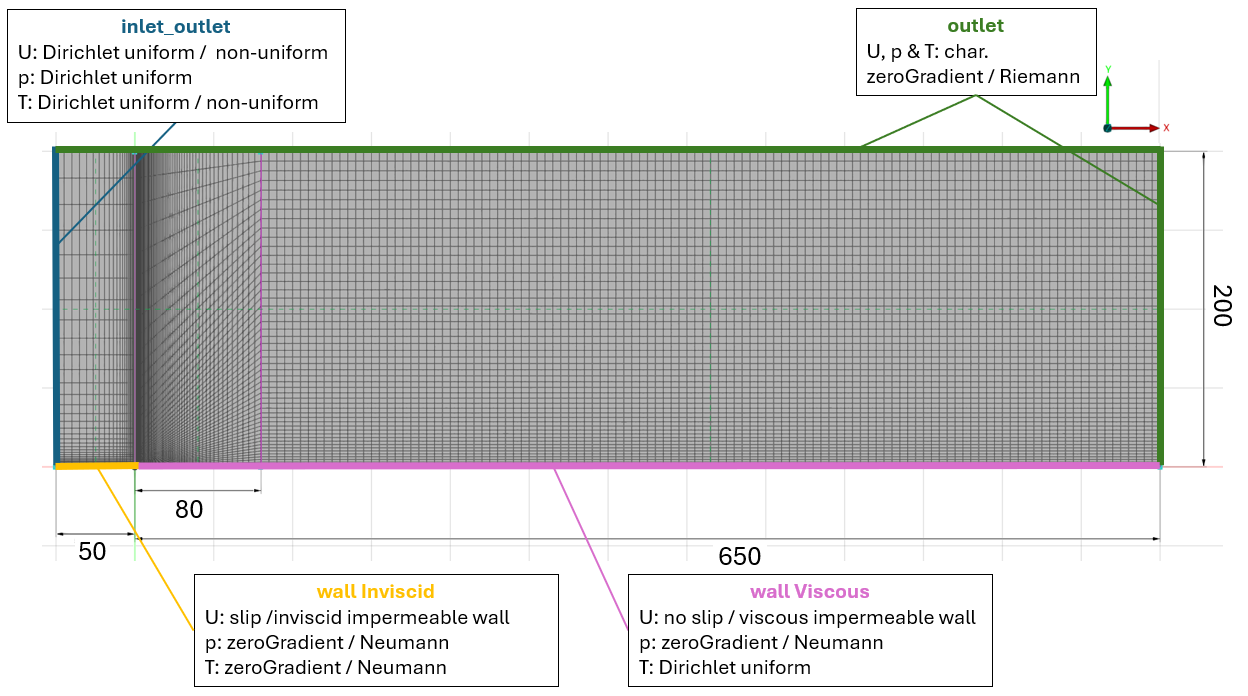
\includegraphics[width=\linewidth,height=.62\textheight,keepaspectratio]{07_Error_Isolation_Results/Figures/WallFunctions/M6Tw025_y+_100_mesh.png}
    \caption{Conventional wall-function mesh for M6Tw025 with nominal first-cell location $y_1^+\approx100$ at the comparison station. Streamwise refinement and a smaller first-cell height resolve the leading-edge region; the wall-normal spacing increases smoothly over the first $80\,\mathrm{mm}$.}
    \label{fig:WF:mesh}
\end{figure}

\begin{figure}[H]
    \centering
    % Figure provenance (WSL; absolute paths):
    %   Figure: /mnt/c/Users/MichaelGnadlinger/OneDrive - Hypersonica/Hypersonica Team - Documents/02 Technical/03 Flight physics/16 Theses/2026/01 Gnadl/Docs_and_Presentations/Thesis_tex/thesis/07_Error_Isolation_Results/Figures/WallFunctions/y+_40_M6Tw025_LiWF_constant.png
    %   Python script: Not applicable: direct ParaView postprocessing screenshot (confirmed by author).
    %   Data / simulation roots (high-level):
    %     /home/mgnadlinger/Xue_et_al/flat_plate/legacy/M6Tw025/LiNeumann_6e-1
    %   Note: No separate export file or plotting script: retained screenshot is at the figure path above.
    %   Note: Association with the listed legacy Li case is inferred from matching mesh geometry and wall-y+
    %     distribution; the original ParaView case path was not recorded.
    % End figure provenance.
    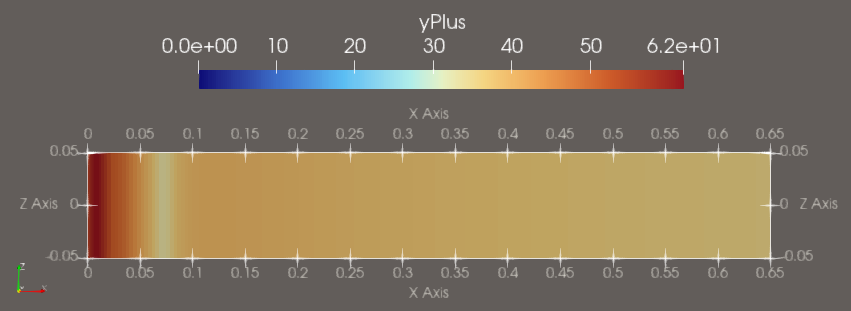
\includegraphics[width=0.7\linewidth,height=.30\textheight,keepaspectratio]{07_Error_Isolation_Results/Figures/WallFunctions/y+_40_M6Tw025_LiWF_constant.png}
    \par\medskip
    % Figure provenance (WSL; absolute paths):
    %   Figure: /mnt/c/Users/MichaelGnadlinger/OneDrive - Hypersonica/Hypersonica Team - Documents/02 Technical/03 Flight physics/16 Theses/2026/01 Gnadl/Docs_and_Presentations/Thesis_tex/thesis/07_Error_Isolation_Results/Figures/WallFunctions/y+_40_M6Tw025_LiWF_smooth.png
    %   Python script: Not applicable: direct ParaView postprocessing screenshot (confirmed by author).
    %   Data / simulation roots (high-level):
    %     /home/mgnadlinger/Xue_et_al/flat_plate/legacy/M6Tw025/LiNeumann_6e-1_smooth
    %   Note: No separate export file or plotting script: retained screenshot is at the figure path above.
    %   Note: Association with the listed legacy Li case is inferred from matching mesh geometry and wall-y+
    %     distribution; the original ParaView case path was not recorded.
    % End figure provenance.
    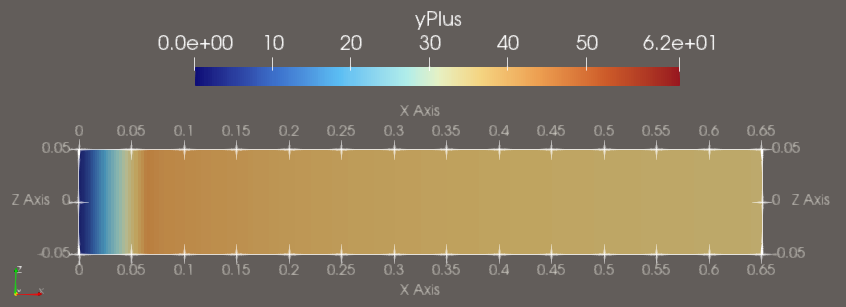
\includegraphics[width=0.7\linewidth,height=.30\textheight,keepaspectratio]{07_Error_Isolation_Results/Figures/WallFunctions/y+_40_M6Tw025_LiWF_smooth.png}
    \caption{Wall-unit first-cell location along the M6Tw025 plate for a nominal $y_1^+\approx40$ Li wall-function mesh. A constant physical first-cell height (top) produces elevated $y_1^+$ near the leading edge. A smooth increase of first-cell height over the first $80\,\mathrm{mm}$ (bottom) reduces this upstream excursion.}
    \label{fig:WF:mesh_constant_smooth}
\end{figure}

Figures~\ref{fig:WF:Li-LowHM3_conventional_mesh}--\ref{fig:WF:Griffin-M6Tw025_conventional_mesh} show the resulting wall heat-flux and shear-stress errors. All curves use the signed relative error to the respective DNS reference at the matched \(Re_{\delta2}\) station (see Section~\ref{subsec:evaluation:matching-station}). The dashed lines show the wall-resolved SA result at the same station as presented and discussed in Section~\ref{sec:comparative:zpg:wall-resolved-baselines}. Around the DNS reference value for th heat-flux and shear stress, the shading marks a $\pm5\%$ error band (as selected in Section~\ref{sec:evaluation:success-criteria}). The horizontal axis shows the actual, calculated first-cell $y_1^+$ at the matched station on these conventional meshes, so each point represents a different CFD simulation with the only change being the first-cell height in the sampling region of the used mesh.
\par\medskip

From Figures~\ref{fig:WF:Li-LowHM3_conventional_mesh}--\ref{fig:WF:Griffin-M6Tw025_conventional_mesh}  it is immediatly visible that the wall-function results are highly sensitive to the first-cell height. But the errors are not monotonic with increasing $y_1^+$, but instead exhibit a pronounced different behaviour in the sublayer region, the buffer and the log-layer region of the cases. The wall-function error bands are also substantially larger than the corresponding a-priori closure variations identified in Section~\ref{subsec:erriso:apriori-results}. Griffin gives signed shear-stress errors of approximately \(-20\%\) to \(+8\%\) and heat-flux errors of \(-16\%\) to \(+12\%\). Over the same cases and sampling-height interval, the Li wall function gives respective shear-stress errors of approximately \(-7\%\) to \(+14\%\) and heat-flux errors of \(-6\%\) to \(+27\%\). But for an engineering context, the high sensitivity of the wall-function results to the first-cell height is arguably more concerning than the absolute error magnitude because it introduces a substantial uncertainty and not a clear bias.
\par\medskip

Looking at the sub-layer region, the wall-function results approach the wall-resolved baseline to within the closure accuracy as expected. Looking at Li's previously found closure behaviour where at \(y^+ = 1\) the wall-function closure error is basically zero (see a-priori result for M6Tw025 in Figure~\ref{fig:wall-closure:a-priori-Li-M6Tw025} and LowH\_M3 in Figure \ref{fig:wall-closure:a-priori-Li-LowHM3}), the wall-function CFD results are also very close to the wall-resolved baseline (see conventional mesh CFD result for M6Tw025 in Figure~\ref{fig:WF:Li-M6Tw025_conventional_mesh} and LowH\_M3 in Figure \ref{fig:WF:Li-LowHM3_conventional_mesh}). The same findings also apply to the Griffin wall-function results where for both cases the a-priori closure assessment in Section~\ref{subsec:erriso:apriori-results} shows a low-$y^+$ closure discrepancy of about $-5\%$ for the wall heat-flux (see a-priori result for M6Tw025 in Figure~\ref{fig:wall-closure:a-priori-Griffin-M6Tw025} and LowH\_M3 in Figure \ref{fig:wall-closure:a-priori-Griffin-LowHM3}), which is also reflected in the deviation of wall-function CFD results from the wall-resolved baseline (see conventional mesh CFD result for M6Tw025 in Figure~\ref{fig:WF:Griffin-M6Tw025_conventional_mesh} and LowH\_M3 in Figure \ref{fig:WF:Griffin-LowHM3_conventional_mesh}).
\par\medskip

Beyond the sublyer, reaching into the buffer layer, the wall-function CFD results do not follow this behaviour where the whole error can be explained through the closure error alone. Rather it is clear that the wall-function CFD results are not only affected by the closure discrepancy, but also by additional error sources. The cause for this behaviour beyond the sublayer is analysed and examined in the next step, where the internal-face fluxues of momentum and energy where compared to the wall-resolved results, and found in the spatial discretization.
\par\medskip

On the even higher $y^+$ conventional meshes, reaching the log-layer and beyond, a sharp reduction in the wall-function CFD error is observed. This reduction does not necessarily indicate a better wall-function performance, but rather indicates a different error sources, that happens to cancel some of the closure discrepancy. In Figure~\ref{fig:WF:Griffin-M6Tw025_conventional_mesh} for example the relative error becomes highly negative, instead of cancelling out to zero. And this behvior in the log-layer and beyond also, as in the buffer layer, do not follow the a-priori seen closure discrepancy. But it is a nice indication why Li et al  found a good agreement of their wall-function CFD results with the DNS reference, because for their validation cases they used a conventional mesh with a first-cell height of \(y^+_1 = 4, 8 \) and then for their cases comfortly in the log-layer \(y^+_1 = 104, 133, 156, 200\) \cite[Figures 17--20 and 23--24]{li2025WF}. Li et al. claim "[...] and it is also essential to avoid them [first grid points] falling into the bufferlayer when using the wall function method." \cite[p. 61]{li2025WF}. So in their analysis they avoided the regions with high sensitivity and large errors, but attributed it to the wrong cause. Griffin et al. use \(y_m=0.3\delta\) for their principal wall-flux comparisons, but also reduce the matching height during WMLES mesh refinement, reaching the buffer region in the lower-Reynolds-number channel case~\cite[Section~4.1]{griffin2023WF}. Their study therefore does not support a blanket exclusion of buffer-layer sampling. As discussed in Section~\ref{subsec:wall-functions:griffin:validation-scope}, those matching-height and LES-resolution studies differ from the present conventional RANS mesh sweeps.

\begin{figure}[H]
    \centering
    % Figure provenance (WSL; absolute paths):
    %   Figure: /home/mgnadlinger/WF_validation/LowH_M3/validation/outputs/plots/li_sa_dns_station_relative_error.png
    %   Python script:
    %     /home/mgnadlinger/WF_validation/LowH_M3/validation/scripts/plot_wall_flux_sweeps.py
    %   Data / simulation roots (high-level):
    %     /home/mgnadlinger/WF_validation/LowH_M3/Li_SA
    %     /home/mgnadlinger/WF_validation/LowH_M3/wall_resolved/SA/LowH_M3
    %     /home/mgnadlinger/WF_validation/LowH_M3/Digitizations
    %   Note: Thesis image removes the 128-pixel title strip from the source export.
    % End figure provenance.
    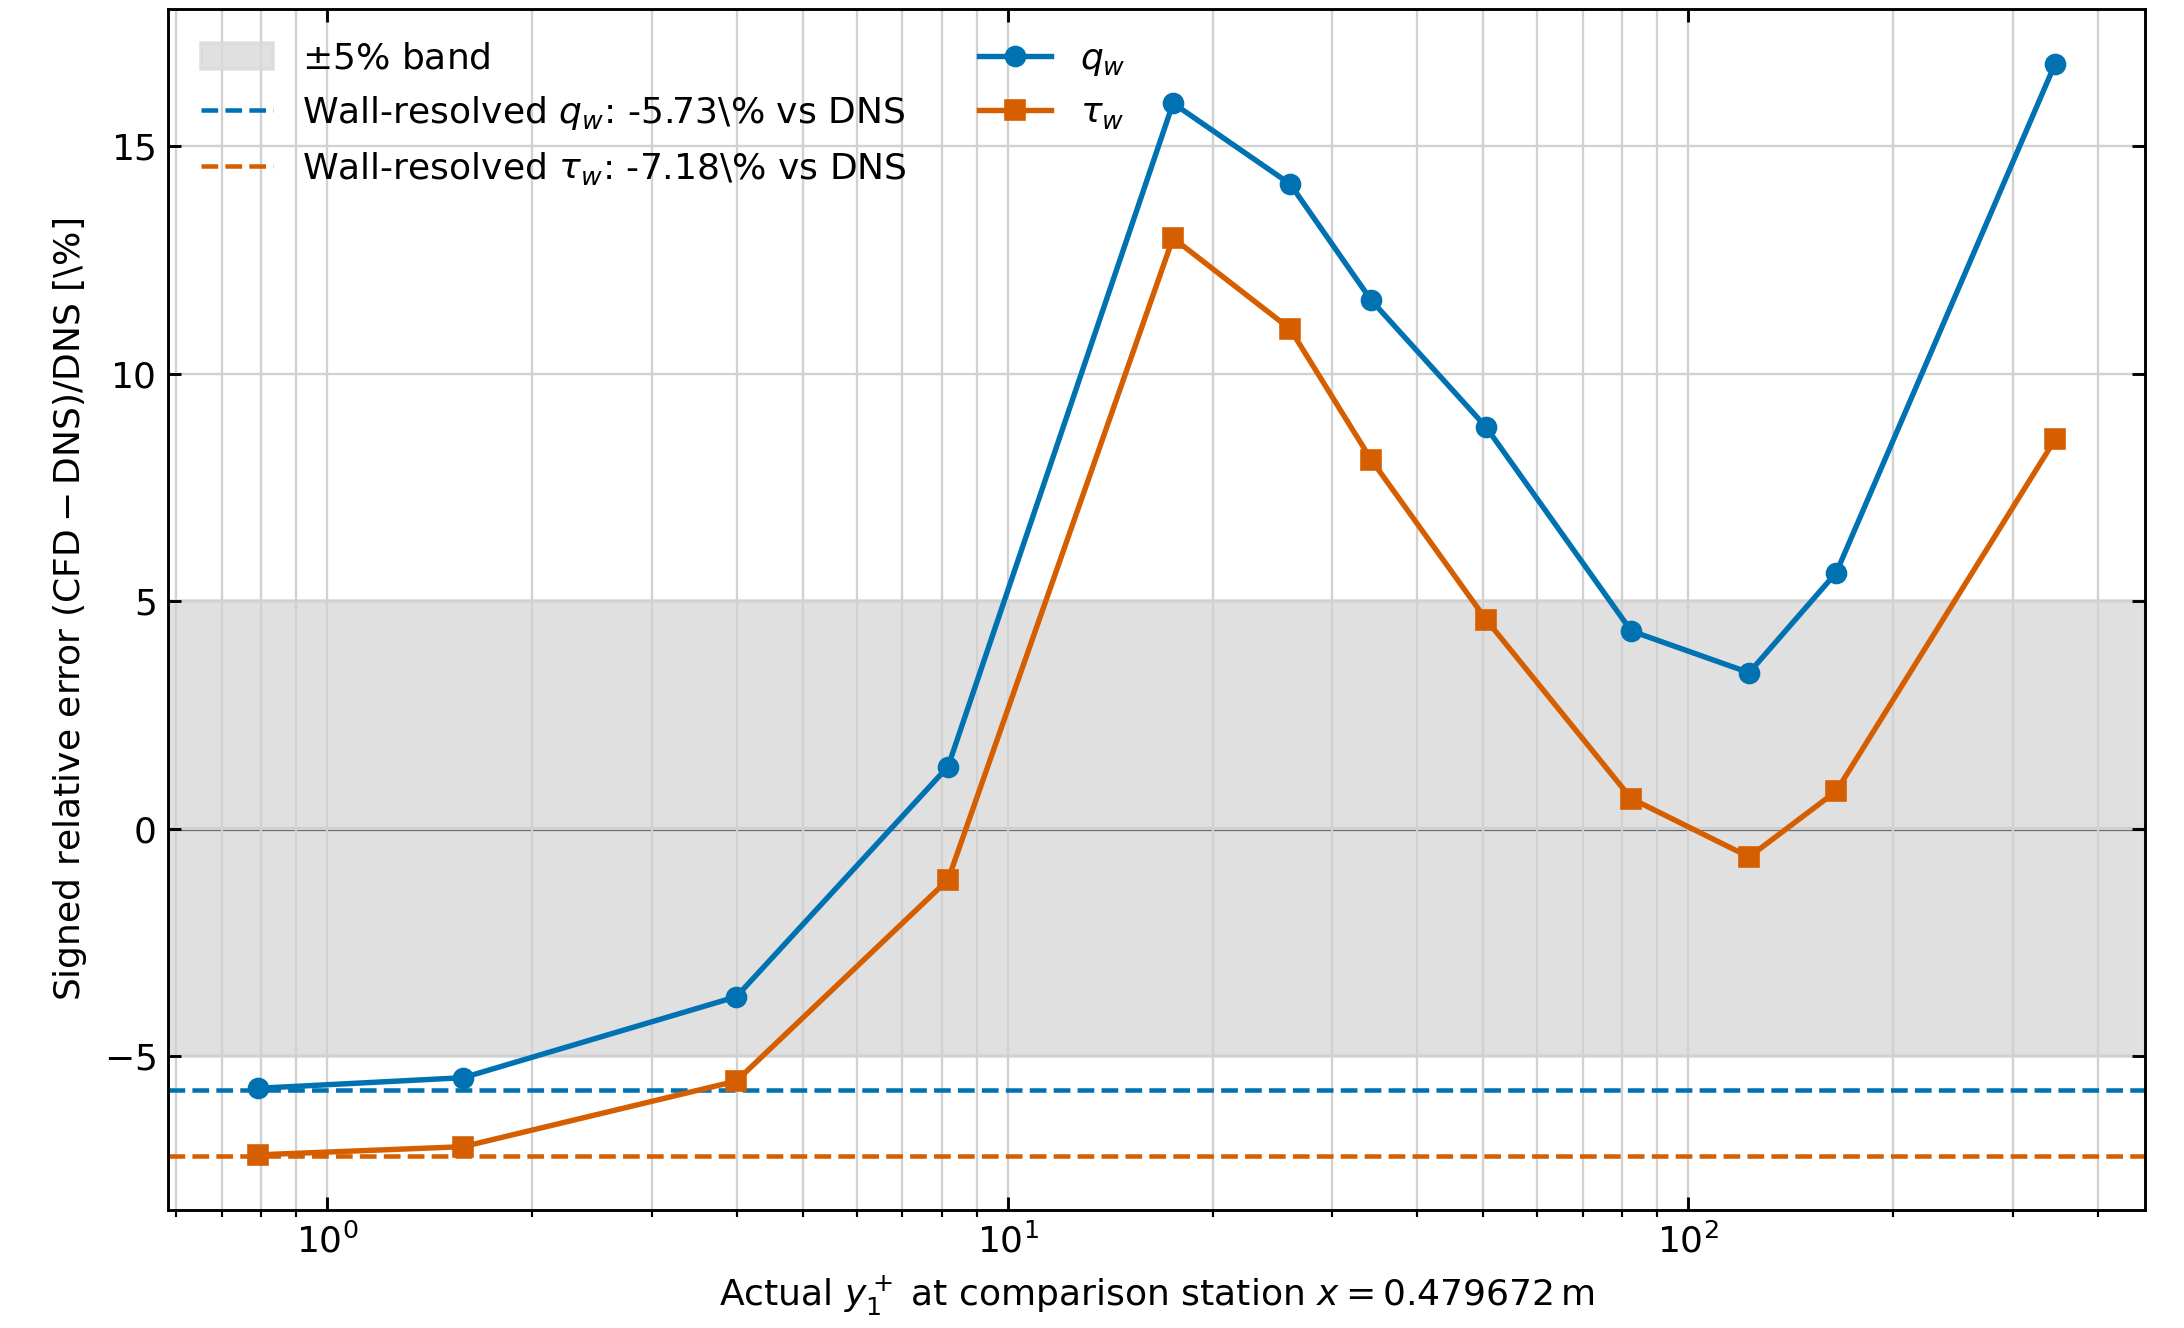
\includegraphics[width=\linewidth,height=.62\textheight,keepaspectratio]{07_Error_Isolation_Results/Figures/WallFunctions/04_ConvMesh_Li_LowHM3.png}
    \caption{Li wall-function CFD with SA on conventional meshes for LowH\_M3: signed errors in wall heat-flux $q_w$ and shear stress $\tau_w$ relative to DNS, evaluated at $x=0.479672\,\mathrm{m}$ against the actual first-cell $y_1^+$. Dashed lines denote the wall-resolved SA errors; shading marks $\pm5\%$ relative to DNS.}
    \label{fig:WF:Li-LowHM3_conventional_mesh}
\end{figure}

\begin{figure}[H]
    \centering
    % Figure provenance (WSL; absolute paths):
    %   Figure: /home/mgnadlinger/WF_validation/LowH_M3/validation/outputs/plots/griffin_sa_dns_station_relative_error.png
    %   Python script:
    %     /home/mgnadlinger/WF_validation/LowH_M3/validation/scripts/plot_wall_flux_sweeps.py
    %   Data / simulation roots (high-level):
    %     /home/mgnadlinger/WF_validation/LowH_M3/Griffin_SA
    %     /home/mgnadlinger/WF_validation/LowH_M3/wall_resolved/SA/LowH_M3
    %     /home/mgnadlinger/WF_validation/LowH_M3/Digitizations
    % End figure provenance.
    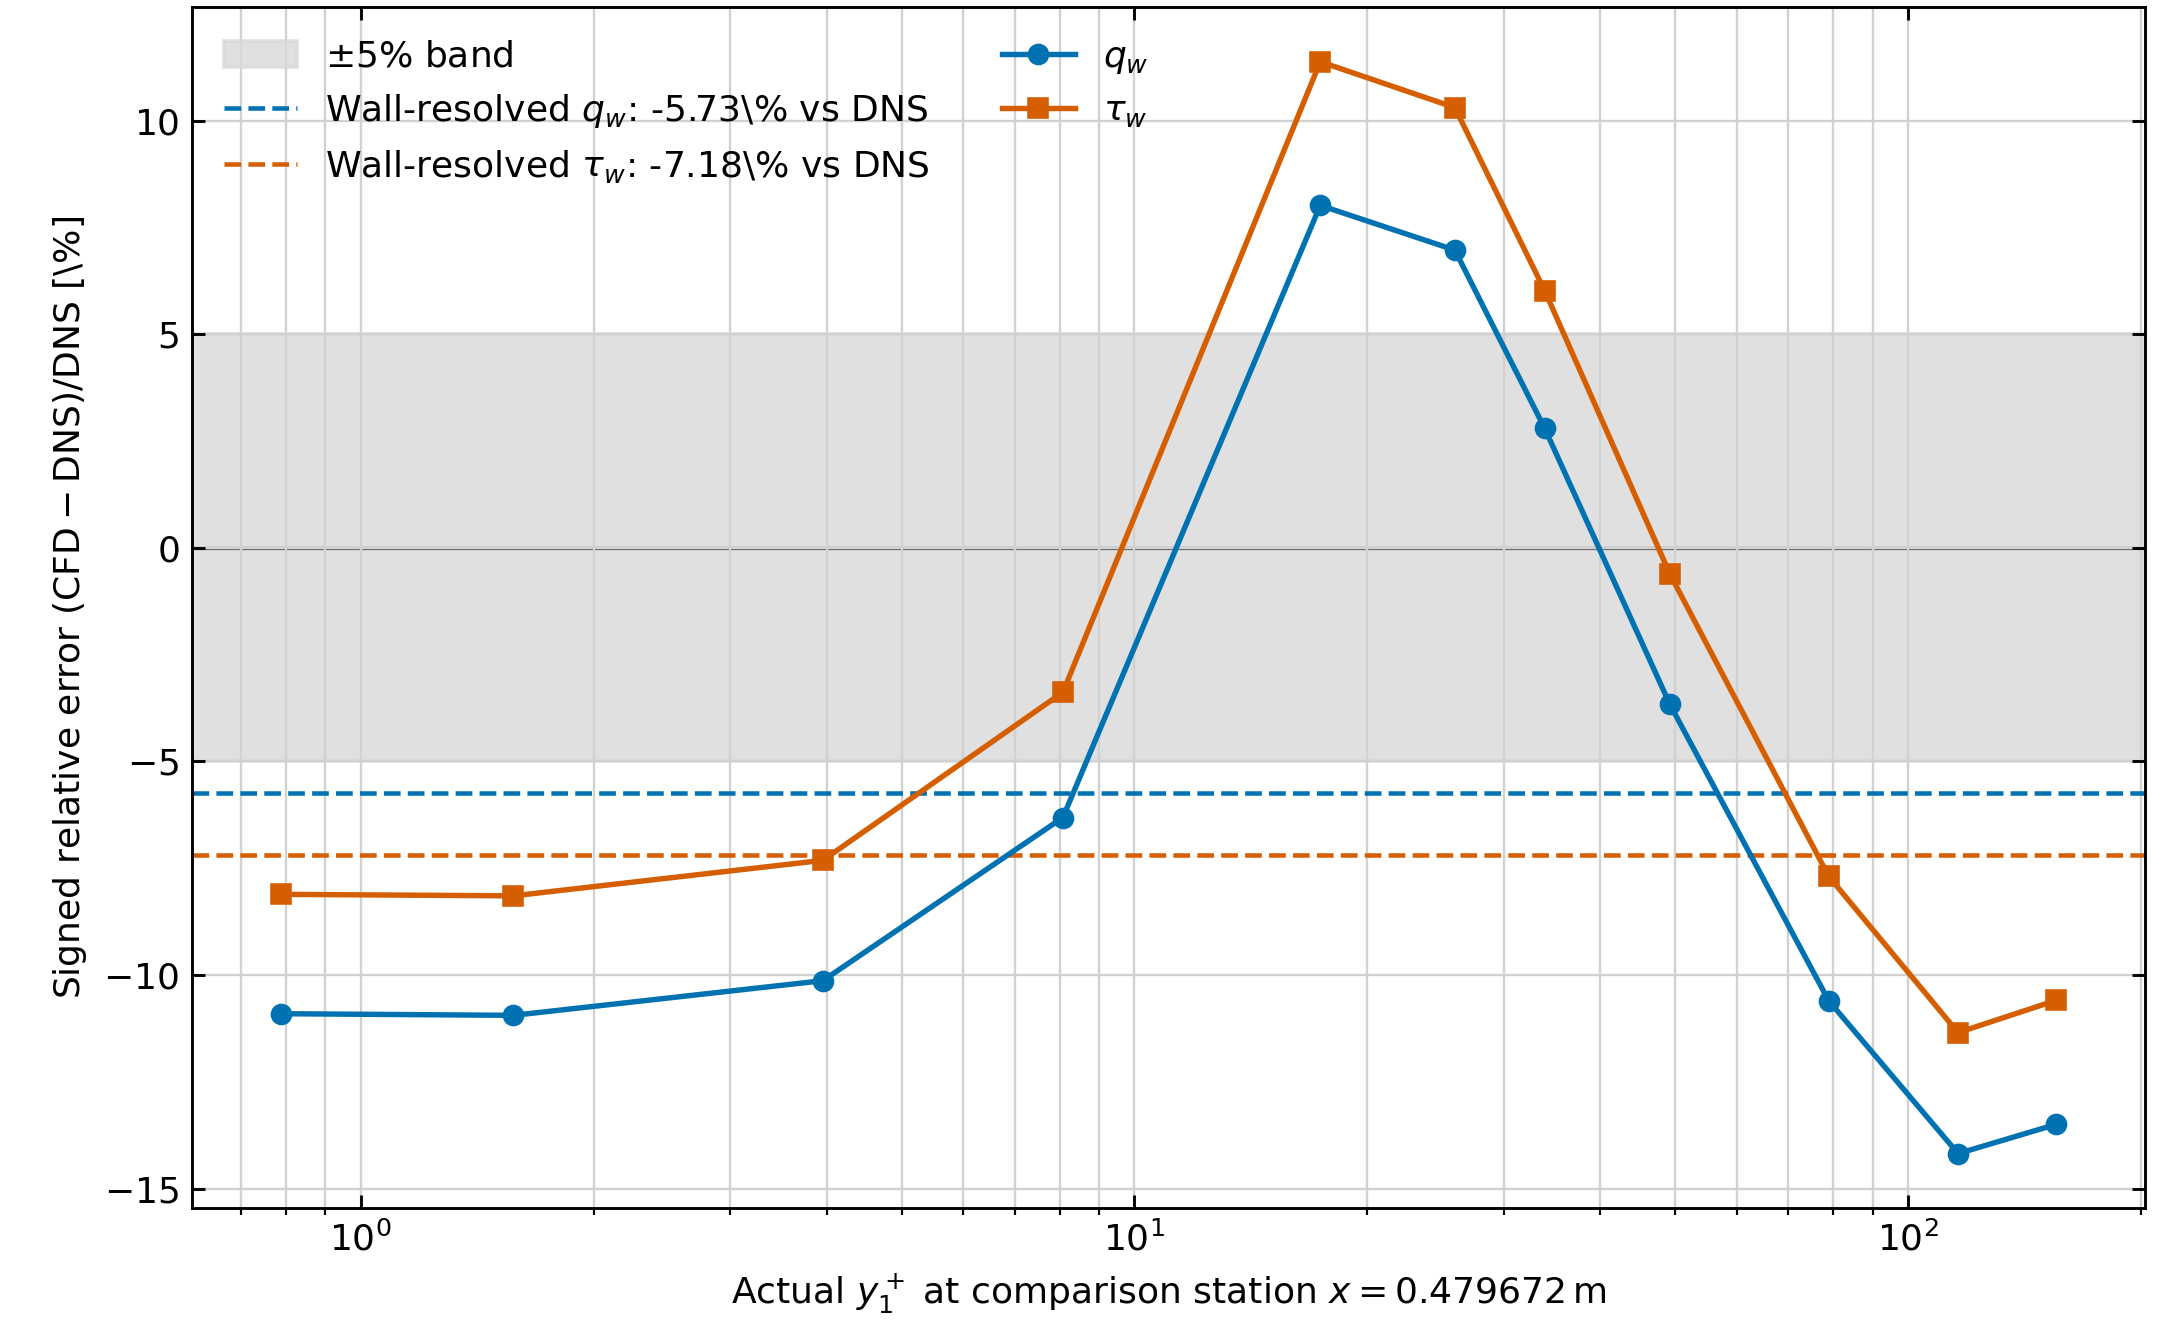
\includegraphics[width=\linewidth,height=.62\textheight,keepaspectratio]{07_Error_Isolation_Results/Figures/WallFunctions/04_ConvMesh_Griffin_LowHM3.png}
    \caption{Griffin wall-function CFD with SA on conventional meshes for LowH\_M3. Wall heat-flux and shear-stress errors use the same DNS normalization and comparison station as Figure~\ref{fig:WF:Li-LowHM3_conventional_mesh}. Dashed lines denote the wall-resolved baseline; shading marks $\pm5\%$ relative to DNS.}
    \label{fig:WF:Griffin-LowHM3_conventional_mesh}
\end{figure}

\begin{figure}[H]
    \centering
    % Figure provenance (WSL; absolute paths):
    %   Figure: /home/mgnadlinger/Xue_et_al/flat_plate/M6Tw025/validation/outputs_Li_SA/group1_wall_flux_relative_error_vs_yplus.png
    %   Python script:
    %     /home/mgnadlinger/Xue_et_al/flat_plate/M6Tw025/validation/plot_wall_fluxes_and_figure6.py
    %   Data / simulation roots (high-level):
    %     /home/mgnadlinger/Xue_et_al/flat_plate/M6Tw025/Li_SA
    %     /home/mgnadlinger/Xue_et_al/flat_plate/M6Tw025/Li_SA/SA_Prt0p9_baseline
    %     /home/mgnadlinger/Xue_et_al/flat_plate/M6Tw025/Digitizations
    %     /home/mgnadlinger/Zhang_DNS_ZPGFP/References/Data
    %   Note: Thesis image removes the 128-pixel title strip from the source export.
    % End figure provenance.
    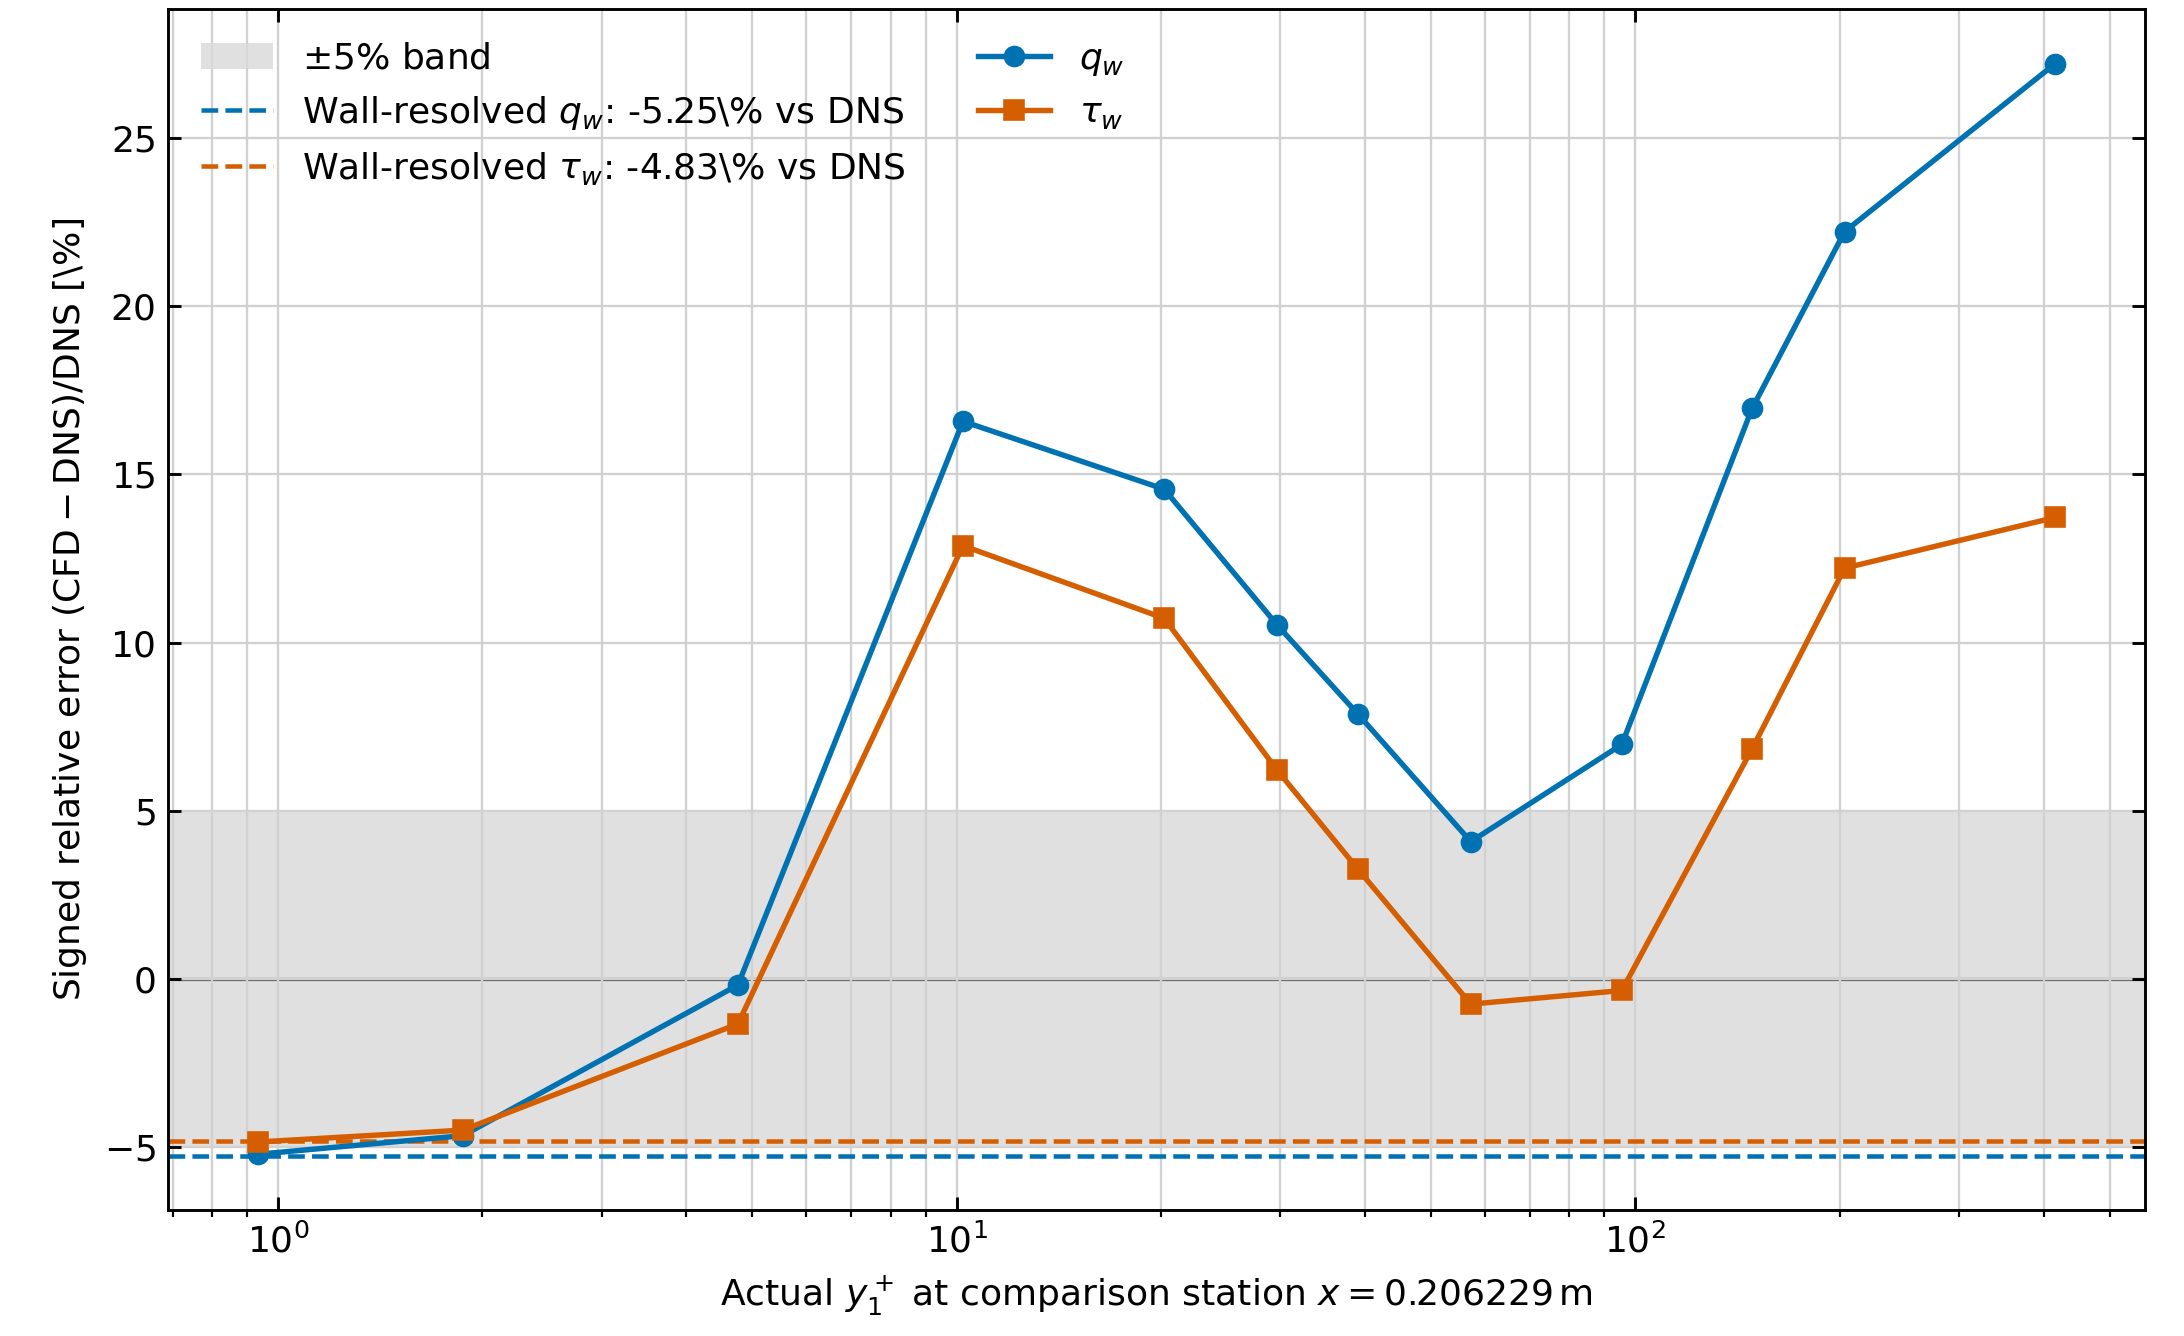
\includegraphics[width=\linewidth,height=.62\textheight,keepaspectratio]{07_Error_Isolation_Results/Figures/WallFunctions/04_ConvMesh_Li_M6Tw025.png}
    \caption{Li wall-function CFD with SA on conventional meshes for M6Tw025: signed wall heat-flux and shear-stress errors relative to DNS at $x=0.206229\,\mathrm{m}$ against the actual first-cell $y_1^+$. Dashed lines denote the wall-resolved SA errors; shading marks $\pm5\%$ relative to DNS.}
    \label{fig:WF:Li-M6Tw025_conventional_mesh}
\end{figure}

\begin{figure}[H]
    \centering
    % Figure provenance (WSL; absolute paths):
    %   Figure: /home/mgnadlinger/Xue_et_al/flat_plate/M6Tw025/validation/outputs_Griffin_SA/group1_wall_flux_relative_error_vs_yplus.png
    %   Python script:
    %     /home/mgnadlinger/Xue_et_al/flat_plate/M6Tw025/validation/plot_wall_fluxes_and_figure6.py
    %   Data / simulation roots (high-level):
    %     /home/mgnadlinger/Xue_et_al/flat_plate/M6Tw025/Griffin_SA
    %     /home/mgnadlinger/Xue_et_al/flat_plate/M6Tw025/Griffin_SA/SA_Prt0p9_baseline
    %     /home/mgnadlinger/Xue_et_al/flat_plate/M6Tw025/Digitizations
    %     /home/mgnadlinger/Zhang_DNS_ZPGFP/References/Data
    % End figure provenance.
    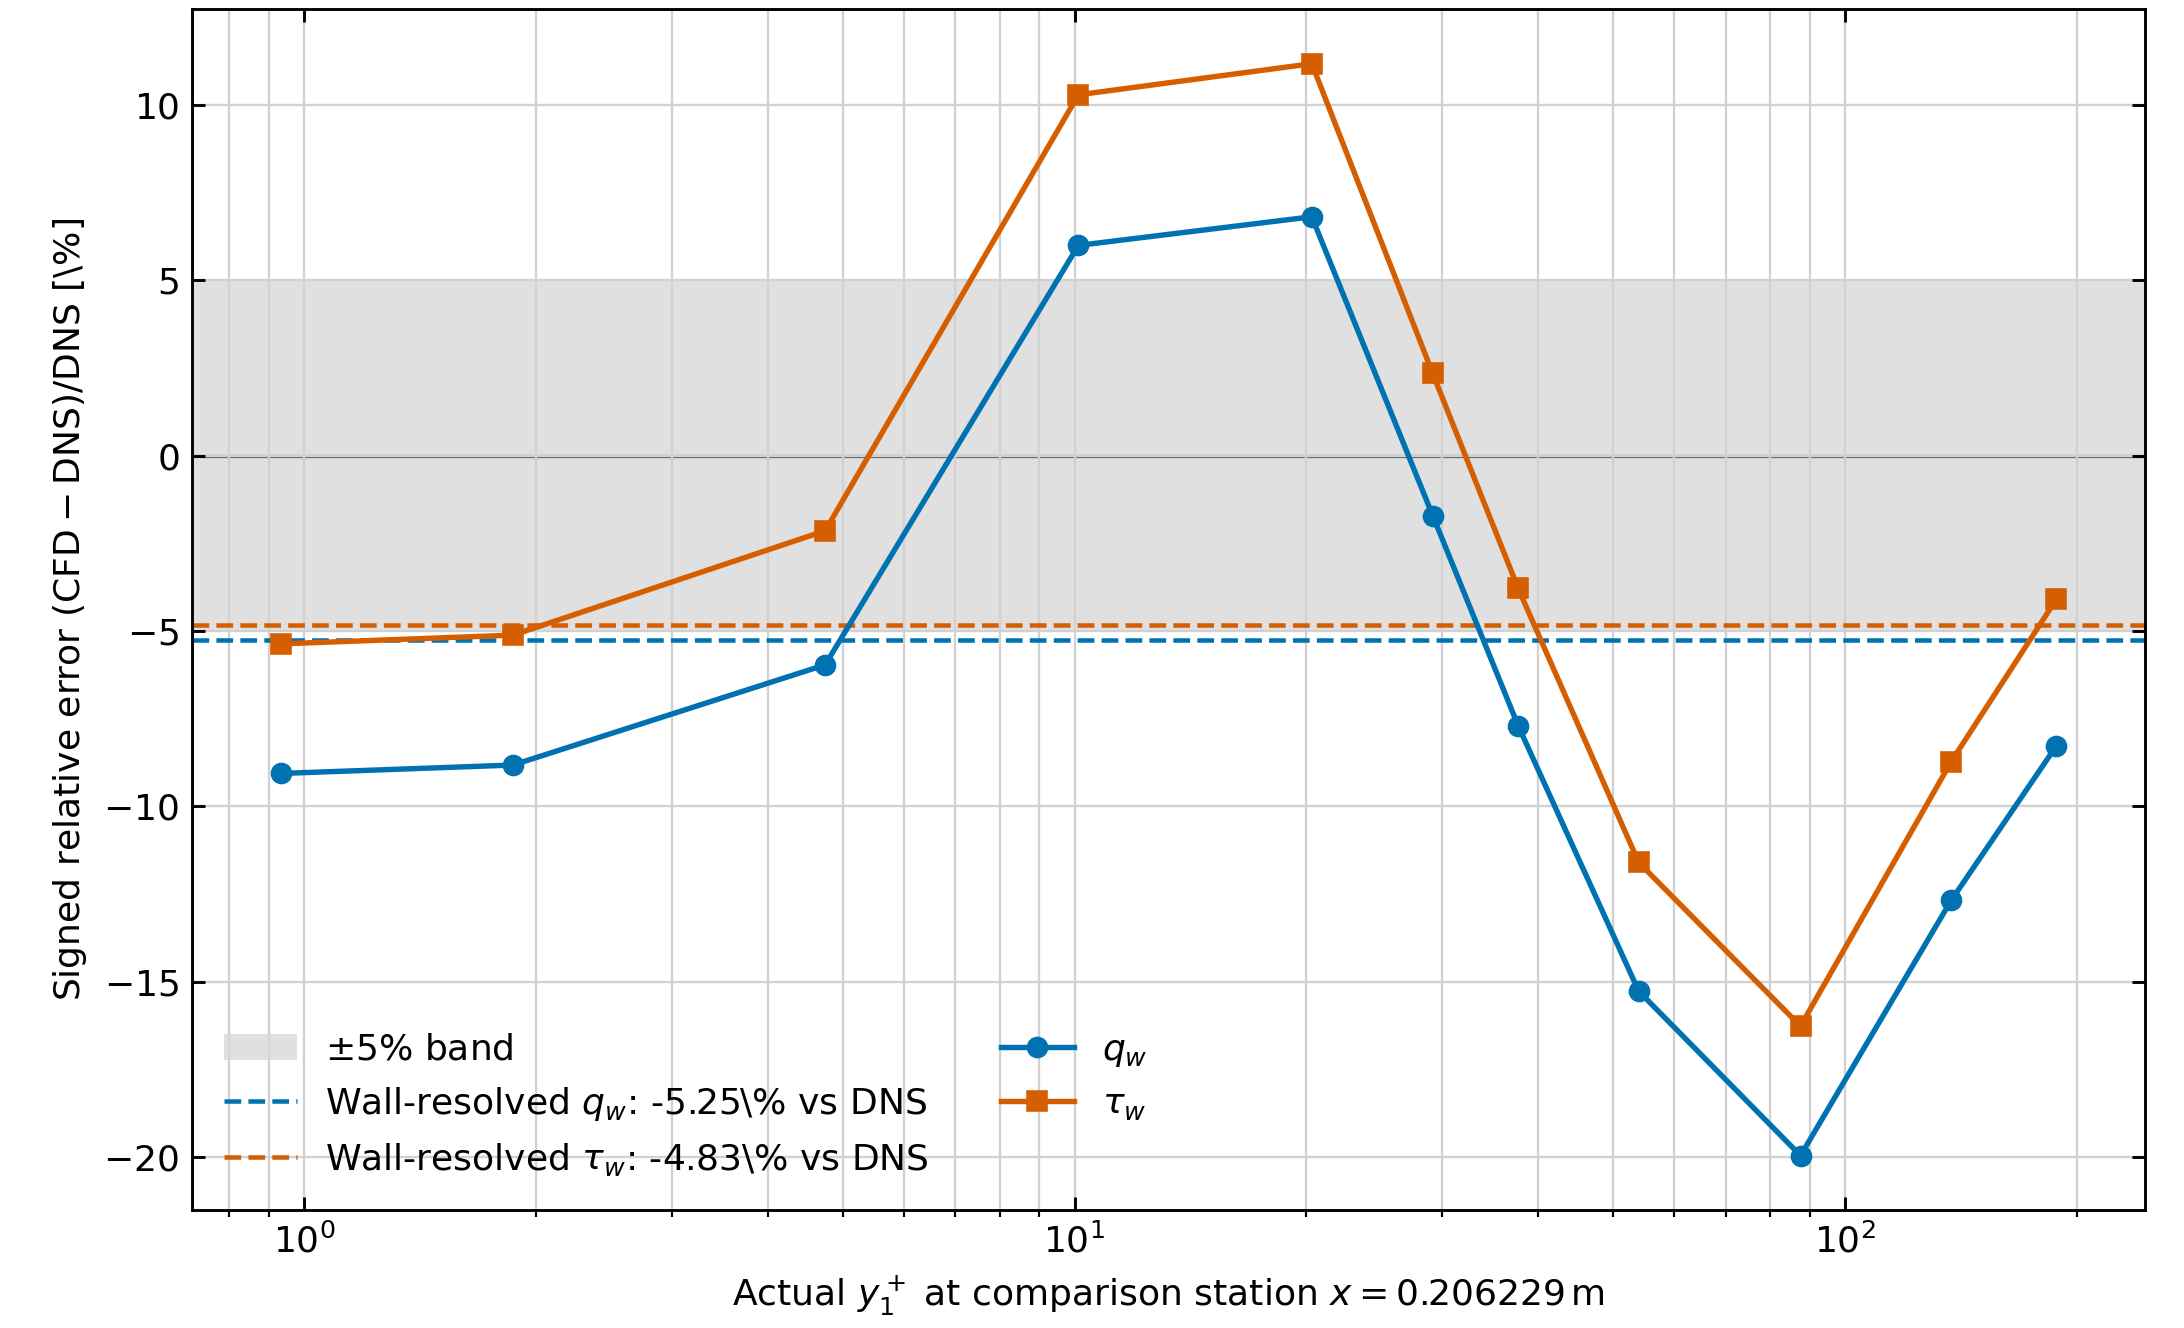
\includegraphics[width=\linewidth,height=.62\textheight,keepaspectratio]{07_Error_Isolation_Results/Figures/WallFunctions/04_ConvMesh_Griffin_M6Tw025.png}
    \caption{Griffin wall-function CFD with SA on conventional meshes for M6Tw025, using the DNS normalization and station of Figure~\ref{fig:WF:Li-M6Tw025_conventional_mesh}. Dashed lines denote the wall-resolved baseline; shading marks $\pm5\%$ relative to DNS.}
    \label{fig:WF:Griffin-M6Tw025_conventional_mesh}
\end{figure}

\subsection{Internal-face errors and a wall-normal spacing criterion}
\label{subsec:comparative:zpg:mesh-criterion}

For the FVM CFD, the numerical framework, is described in Section~\ref{sec:numerical-framework:discretization} and
distinguishes convective reconstruction from viscous flux evaluation. The direct wall-flux delivery of the wall-functions, as described in Section~\ref{subsec:wall-functions:direct-flux-delivery}, replaces the gradient-based evaluation at the wall, but gradients and transport coefficients at internal faces must still be approximated from the cell-centre values. For a predominantly streamwise boundary layer flow, neglecting $\partial V/\partial x$ relative to $\partial U/\partial y$ gives
\begin{equation}
    \tau_{xy}\simeq\mu_{\mathrm{eff}}\frac{\partial U}{\partial y},
    \qquad
    q_y=-\kappa_{\mathrm{eff}}\frac{\partial T}{\partial y}.
    \label{eq:erriso:diffusive-face-fluxes}
\end{equation}
Here $\tau_{xy}$ is the effective shear stress and $q_y$ is the effective heat-flux in the positive wall-normal direction. At internal faces parallel to the wall, these fluxes contribute to the discrete momentum and energy balances. As Equation~\ref{eq:erriso:diffusive-face-fluxes} shows, their evaluation relies both on wall-normal gradient approximations as well as interpolation of the effective viscosity $\mu_{\mathrm{eff}}$ and thermal conductivity $\kappa_{\mathrm{eff}}$ at the face location. Errors in either can therefore alter the flow field solution, which in turn feeds into the wall-function.
\par\medskip

Figure~\ref{fig:WF:exemplaray_y+10_mesh} visualizes the geometry of these operations on an exemplary conventional coarse wall-function mesh with a first-cell height of $y_1^+=10$ on the left and $y_1^+=30$ on the right. For equal adjacent cell thicknesses, the first centre at $y_1^+=10$ and the next at $y_2^+=30$ surround the internal face at $y_f^+=20$. The full centre separation, which the gradient approximation and coefficient interpolation needs to gap, is thus $h^+=20$. Increasing the first-cell height to $y_1^+=30$ also increases the stencil separation to $y_f^+=h^+=60$. Thus conventional coarsening changes both the wall-function sampling height and the distance over which internal-face transport is evaluated. The former already isolately evaluated in Section~\ref{sec:comparative:zpg:cross-comparison} and the latter is evaluated in this section.

\begin{figure}[H]
    \centering
    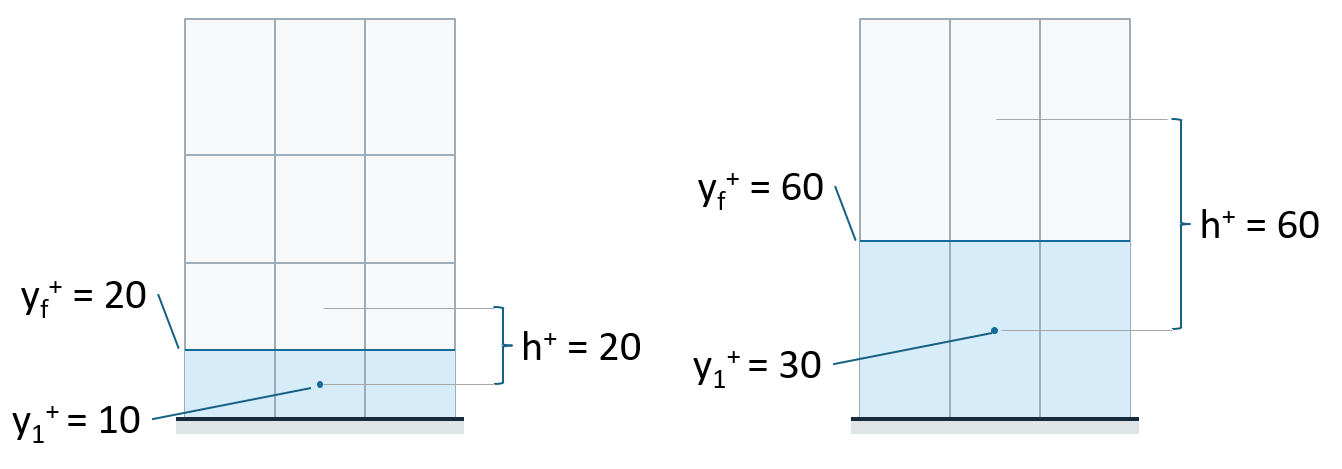
\includegraphics[width=\linewidth,height=.62\textheight,keepaspectratio]{07_Error_Isolation_Results/Figures/Recon/illustration_conv_coarse_mesh.png}
    \caption{Illustrative conventional near-wall meshes. For equal cell thicknesses adjacent to the first internal face, $y_1^+=10$ gives $y_f^+=h^+=20$ (left), while $y_1^+=30$ gives $y_f^+=h^+=60$ (right). Here $h^+$ is the full centre separation. The lower cell extends from the wall to the face, establishing an upper geometric link between the centre spacing $h^+$ and cell height of $h^+=y_f^+$.}
    \label{fig:WF:exemplaray_y+10_mesh}
\end{figure}

Figure~\ref{fig:WF:exemplaray_y+10_reconstruction_error} uses the M6Tw025 DNS temperature profile to illustrate a potential limitation of second-order accurate internal-face gradient reconstruction in a hypersonic cold-wall boundary layer. For the symmetric two-centre stencil considered here, the second-order accurate face-gradient approximation is the slope of a linear secant through the neighbouring cell-centre values. In this example, the secant connects the temperatures at $y^+=10$ and $30$, while the required gradient is the tangent slope at $y_f^+=20$. The pronounced cold-wall temperature peak causes substantial variation in curvature across this coarse stencil, and the two slopes differ visibly. Thus even a symmetric, second-order accurate approximation can poorly represent the local thermal gradient. This example illustrates the mechanism, while the spacing analysis below quantifies it over the profile. Here second-order accuracy refers to the leading error scaling with the square of the centre separation, not to a quadratic interpolating curve.

\begin{figure}[H]
    \centering
    % Figure provenance (WSL; absolute paths):
    %   Figure: /mnt/c/Users/MichaelGnadlinger/.codex/visualizations/2026/09/28/01a0e8e6-c3e6-7e32-a912-308b04eb3ffd/M6Tw025_temperature_profile_clean_600.png
    %   Python script:
    %     /mnt/c/Users/MichaelGnadlinger/.codex/visualizations/2026/09/28/01a0e8e6-c3e6-7e32-a912-308b04eb3ffd/plot_temperature_profile_clean_600.py
    %   Data / simulation roots (high-level):
    %     /home/mgnadlinger/Xue_et_al/flat_plate/M6Tw025/opt_mesh/reference
    %     /home/mgnadlinger/Xue_et_al/flat_plate/M6Tw025/Digitizations
    %   Note: Thesis image is resized and cropped to remove the title.
    % End figure provenance.
    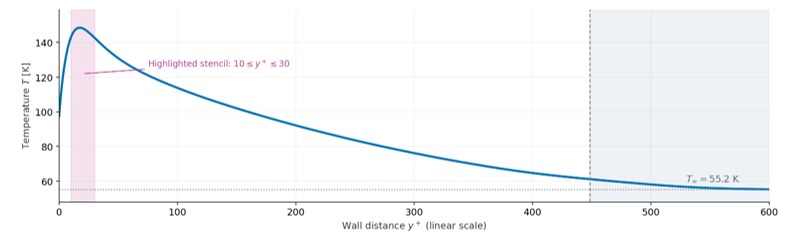
\includegraphics[width=\linewidth,height=.30\textheight,keepaspectratio]{07_Error_Isolation_Results/Figures/Recon/example_M6Tw025_Temperature_profile.png}
    \par\medskip
    % Figure provenance (WSL; absolute paths):
    %   Figure: /mnt/c/Users/MichaelGnadlinger/.codex/visualizations/2026/09/10/01a08aab-7a88-7450-b58c-b4f35bd01e8a/M6Tw025_temperature_full_and_y20.png
    %   Python script:
    %     /mnt/c/Users/MichaelGnadlinger/.codex/visualizations/2026/09/10/01a08aab-7a88-7450-b58c-b4f35bd01e8a/plot_temperature_y20.py
    %   Data / simulation roots (high-level):
    %     /home/mgnadlinger/Xue_et_al/flat_plate/M6Tw025/opt_mesh/reference
    %     /home/mgnadlinger/Xue_et_al/flat_plate/M6Tw025/Digitizations
    %   Note: Thesis image is a resized crop of panel (b), Temperature near the maximum.
    % End figure provenance.
    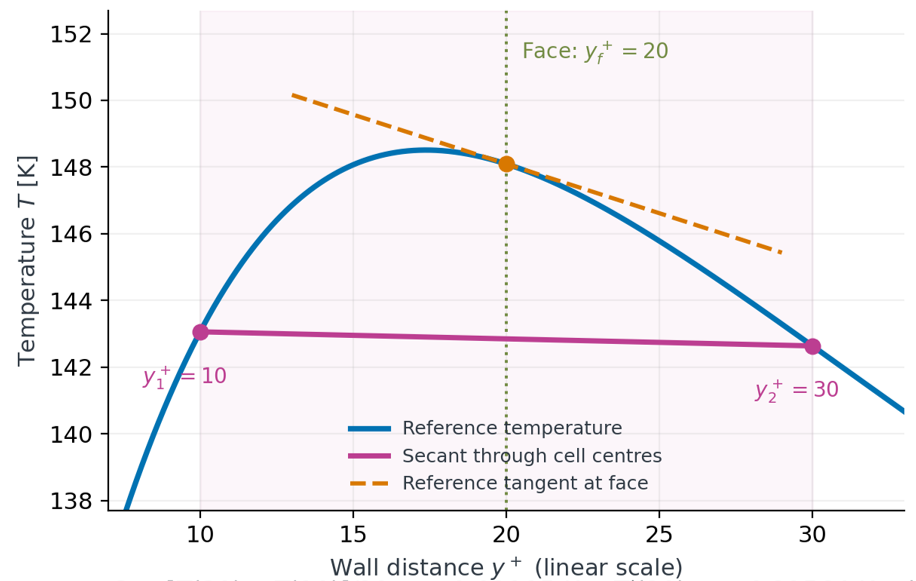
\includegraphics[width=\linewidth,height=.30\textheight,keepaspectratio]{07_Error_Isolation_Results/Figures/Recon/example_M6Tw025_Temperature_zoomed.png}
    \caption{M6Tw025 DNS temperature profile (top) and detail near its maximum (bottom). For the illustrative stencil in Figure~\ref{fig:WF:exemplaray_y+10_mesh}, the purple secant between $y^+=10$ and $30$ differs from the local tangent at the internal face $y_f^+=20$ (orange dashed line). The slopes illustrate the gradient contribution to thermal-diffusion error; the corresponding face flux also depends on the interpolated effective conductivity.}
    \label{fig:WF:exemplaray_y+10_reconstruction_error}
\end{figure}

The two-centre face-gradient approximation of a second-order accurate gradient reconstruction scheme is the slope of the linear secant through the neighbouring profile values:
\begin{equation}
    D_f\phi=\frac{\phi(y_R)-\phi(y_L)}{y_R-y_L}
    =\frac{\phi(y_f+b)-\phi(y_f-a)}{a+b},
    \qquad \phi\in\{T,U\},
\end{equation}
where $a=y_f-y_L$, $b=y_R-y_f$ and $h=a+b$. Unequal spacing introduces a truncation-error contribution $(b-a)\phi''(y_f)/2$. For the symmetric stencil, $a=b=h/2$, however this contribution vanishes and the secant slope approximates the face gradient with second-order accuracy. Taylor expansion expresses the secant slope as the exact tangent slope plus its error:
\begin{equation}
    \frac{\phi(y_f+h/2)-\phi(y_f-h/2)}{h}
    =\phi'(y_f)+\frac{h^2}{24}\phi'''(y_f)+O(h^4),
    \qquad \phi\in\{T,U\}.
    \label{eq:erriso:symmetric-gradient}
\end{equation}
For this symmetric stencil, the leading gradient error therefore depends on the change in curvature, $\phi'''$, rather than curvature alone. Dividing its magnitude by $|\phi'(y_f)|$ and prescribing a relative accuracy of the face gradient $\epsilon$ gives the spacing estimation $h_{\mathrm{grad}}$ for the second order accurate gradient reconstruction on a symmetric stencil as
\begin{equation}
    h_{\mathrm{grad}}\simeq
    \sqrt{24\epsilon\left|\frac{\phi'}{\phi'''}\right|}.
    \label{eq:erriso:gradient-spacing}
\end{equation}
Similarly, for symmetric linear interpolation of a coefficient $\Gamma\in\{\mu_{\mathrm{eff}},\kappa_{\mathrm{eff}}\}$, the face value is approximated by the mean of the two cell-centre values. Its leading error is $h^2\Gamma''(y_f)/8$, giving
\begin{equation}
    h_{\mathrm{interp}}\simeq
    \sqrt{8\epsilon\left|\frac{\Gamma}{\Gamma''}\right|}.
    \label{eq:erriso:coefficient-spacing}
\end{equation}
Equations~\eqref{eq:erriso:symmetric-gradient}--\eqref{eq:erriso:coefficient-spacing} identify the profile derivatives controlling the two operations. The envelopes below evaluate the corresponding finite-stencil errors directly on cubic-interpolation reconstructions of the digital reference profiles. The resulting spacing limits are the maximum centre separation that satisfies a prescribed relative error $\epsilon$ for each operation. 
\par\medskip

Figure~\ref{fig:WF:M6Tw025-profiles} shows exemplary the four profiles of the M6Tw025 case passed through this spacing analysis. DNS supplies M6Tw025 temperature and velocity, the matched wall-resolved SA solution supplies effective viscosity and conductivity. The effective transport properties need to be taken from the wall-resolved SA reference because not published with the DNS profiles. For the subsequent LowH\_M3 mesh design, all profiles come from the wall-resolved SA reference, because of the lack of published high-quality digital DNS data. In the Figure~\ref{fig:WF:M6Tw025-profiles} profiles it is immediatly apparant that the thermal profile present significantly more change in curvature than the velocity profile because of the sharp temperature peak near the wall. As identified in Equation~\eqref{eq:erriso:coefficient-spacing}, the transport coefficients rely on the curvature of the repsetive profiles, rather than the change in curvature, which for the M6Tw025 case has three pronounced regions of high curvature, directly at the wall because of the zero gradient Neumann boundary conditions there, at \(y \approx 0.0025 \mathrm{m}\) and \(y \approx 0.005 \mathrm{m}\) (see Figure~\ref{fig:WF:M6Tw025-profiles} bottom plots). 

\begin{figure}[H]
    \centering
    % Figure provenance (WSL; absolute paths):
    %   Figure: /home/mgnadlinger/Xue_et_al/flat_plate/M6Tw025/opt_mesh/spacing_limits/M6Tw025_DNS_and_wall_resolved_profiles_physical_y_linear.png
    %   Python script:
    %     /home/mgnadlinger/Xue_et_al/flat_plate/M6Tw025/opt_mesh/scripts/plot_requested_profiles.py
    %   Data / simulation roots (high-level):
    %     /home/mgnadlinger/Xue_et_al/flat_plate/M6Tw025/opt_mesh/reference
    %     /home/mgnadlinger/Xue_et_al/flat_plate/M6Tw025/Digitizations
    %     /home/mgnadlinger/Xue_et_al/flat_plate/M6Tw025/Li_SA/SA_Prt0p9_baseline
    %   Note: DNS temperature/velocity and SA effective transport use the frozen reference package; the SA
    %     station is x = 0.206229 m at time 15000.
    % End figure provenance.
    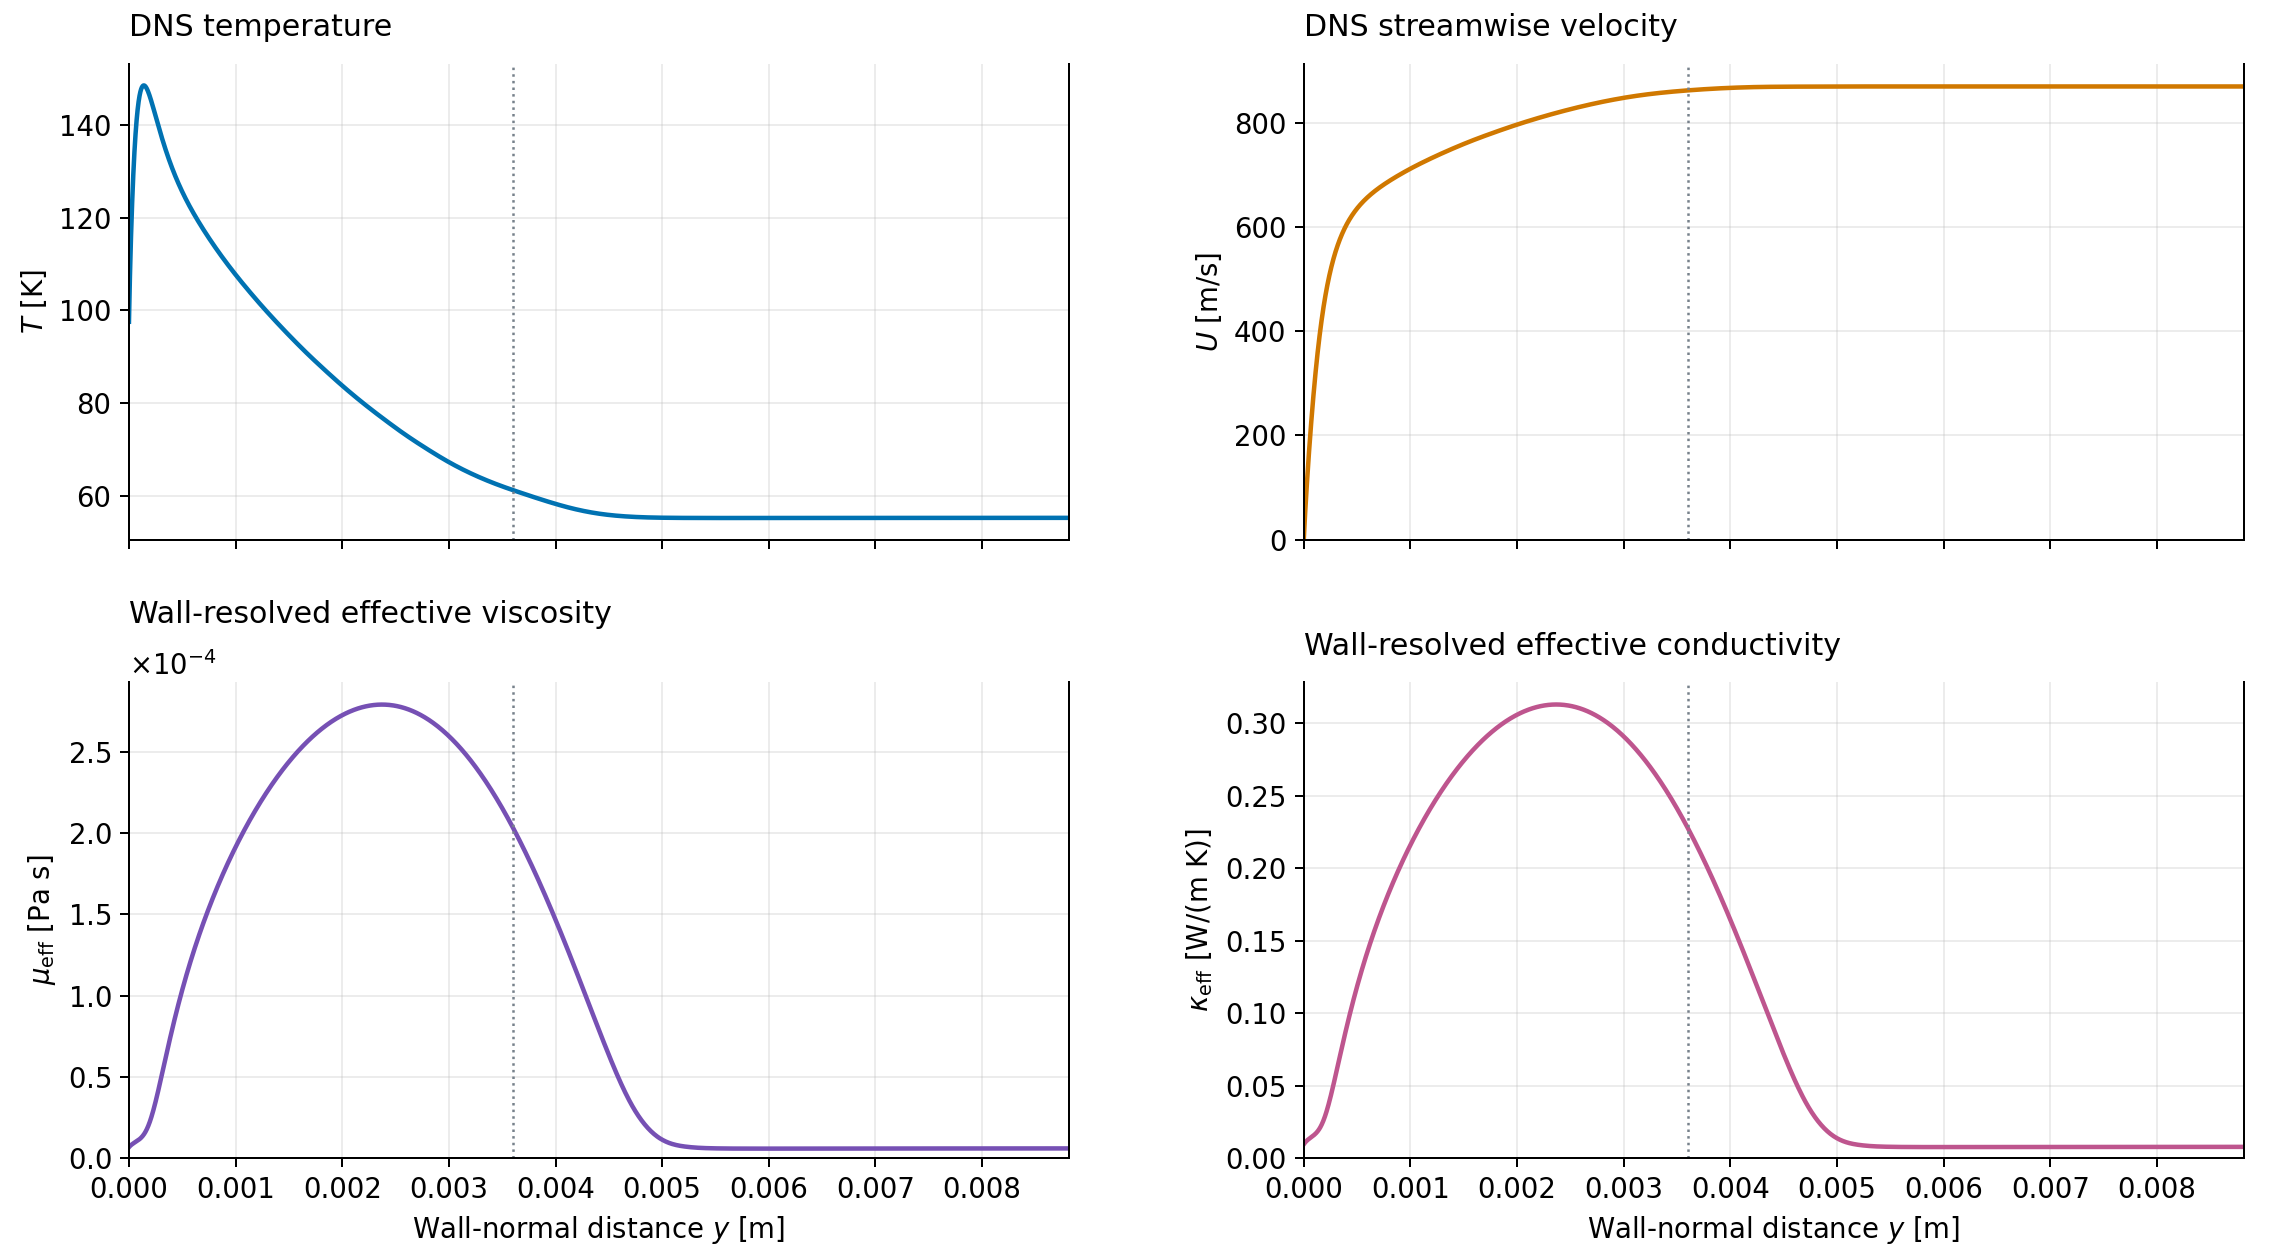
\includegraphics[width=\linewidth,height=.62\textheight,keepaspectratio]{07_Error_Isolation_Results/Figures/Recon/M6Tw025_DNS_BL_profiles_lin-y.png}
    \caption{Profiles underlying the M6Tw025 spacing assessment, plotted against physical wall-normal distance. DNS temperature and velocity are shown above; effective viscosity and thermal conductivity from the matched wall-resolved SA solution are shown below. The temperature maximum and the variation of effective transport motivate separate gradient and coefficient-interpolation criteria.}
    \label{fig:WF:M6Tw025-profiles}
\end{figure}

Using the found Equations \eqref{eq:erriso:gradient-spacing} and \eqref{eq:erriso:coefficient-spacing} that link the cell-centre spacing to the respective gradient reconstruction and interpolation errors, the M6Tw025 profiles of Figure~\ref{fig:WF:M6Tw025-profiles} are analysed. This results in the four individual spacing limits as shown in Figure~\ref{fig:WF:M6Tw025-3pct-envelope-all-quantities}. The resulting envelopes show, the allowable cell spacing $h$, for a given cell face position $y^+_f$ so that the relative errors for the gradient reconstruction or interpolation stay below a given tolerance of e.g. $\epsilon_{max}=3\%$.
\par\medskip

The cell spacing must also adhere to the upper geometric limit of $h^+\leq y_f^+$. At this limit two equal hight cells around a given face have centres at $y_f^+/2$ and $3y_f^+/2$, thus resulting in the lower cell extending all the way from the face to the wall. Thus the full centre separation equals the face-to-wall distance. This is the conventional coarse wall-function mesh geometry illustrated above in Figure~\ref{fig:WF:exemplaray_y+10_mesh}. A limit below this line requires a smaller centre separation at the same face position. a limit reaching it permits that conventional stencil under the selected local criterion. The cap is an adopted mesh constraint, not an error estimate.
\par\medskip

Figure~\ref{fig:WF:M6Tw025-3pct-envelope-all-quantities} shows the individual limits for $\epsilon=0.03$. The temperature-gradient limit has a sharp minimum near the temperature maximum as expected and hypthesized above. The coefficient interpolation and velocity-gradient reconstruction somewhat restrict other parts of the inner layer. At the exact Temperature peak, $T'=0$ thus the relative gradient error of Equations \eqref{eq:erriso:gradient-spacing} appraoches a asymptote - for the M6Tw025 case this is at around $y^+_f\approx 18$, in-line with the plotted temperature profile in Figure~\ref{fig:WF:exemplaray_y+10_reconstruction_error}. The sharp minimum reflects this conditioning as good as the cubic-interpolation of the given profile allows.

\begin{figure}[H]
    \centering
    % Figure provenance (WSL; absolute paths):
    %   Figure: /home/mgnadlinger/Xue_et_al/flat_plate/M6Tw025/opt_mesh/spacing_limits/M6Tw025_finite_spacing_3pct_relative_no_diagnostic_note.png
    %   Python scripts:
    %     /home/mgnadlinger/Xue_et_al/flat_plate/M6Tw025/opt_mesh/scripts/plot_requested_profiles.py
    %     /home/mgnadlinger/Xue_et_al/flat_plate/M6Tw025/opt_mesh/scripts/plot_analysis.py
    %   Data / simulation roots (high-level):
    %     /home/mgnadlinger/Xue_et_al/flat_plate/M6Tw025/opt_mesh/spacing_limits
    %     /home/mgnadlinger/Xue_et_al/flat_plate/M6Tw025/opt_mesh/reference
    %     /home/mgnadlinger/Xue_et_al/flat_plate/M6Tw025/Digitizations
    %     /home/mgnadlinger/Xue_et_al/flat_plate/M6Tw025/Li_SA/SA_Prt0p9_baseline
    %   Note: plot_analysis.py generates the finite-stencil limit tables; plot_requested_profiles.py exports
    %     this cubic-only figure.
    % End figure provenance.
    %   Print-size typography: regenerated at 170 mm width with 10 pt text; exact source table
    %     retained in Figures/Recon/spacing_font_sources/ (script, data and provenance).
    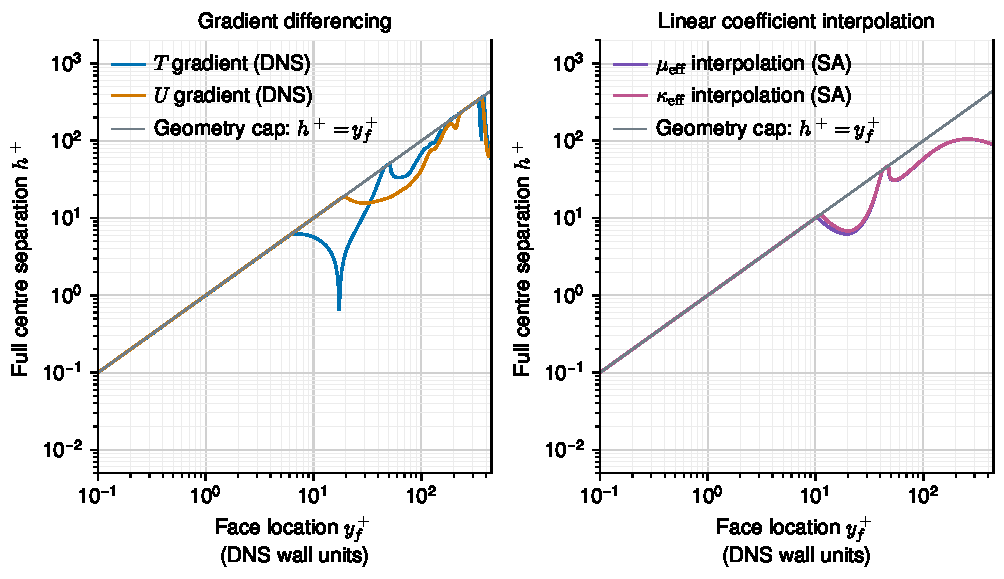
\includegraphics[width=\linewidth]{07_Error_Isolation_Results/Figures/Recon/M6Tw025_3pct_envelope.pdf}
    \caption{M6Tw025 spacing limits at a $3\%$ local component-error tolerance. The allowable full centre separation $h^+$ is plotted against internal-face position $y_f^+$ for centred differencing of DNS temperature and velocity (left) and linear interpolation of wall-resolved SA effective transport (right). Each limit is the first tolerance crossing evaluated on cubic profile reconstructions, capped by the adopted geometric condition $h^+\leq y_f^+$. Both coordinates use DNS wall units.}
    \label{fig:WF:M6Tw025-3pct-envelope-all-quantities}
\end{figure}

To satisfy all four component criteria of Figure~\ref{fig:WF:M6Tw025-3pct-envelope-all-quantities} simultaneously, the allowable spacing is their minimum at each face position, further limited by profile support and the geometric cap. Figure~\ref{fig:WF:M6Tw025-3pct-envelope-combined} is the resulting $3\%$ envelope. It converts the separate operator restrictions into a single wall-normal spacing requirement. Near the cold-wall temperature maximum, its large separation from $h^+=y_f^+$ quantifies why the conventional coarse stencil is inadequate and how much smaller the centre separation must be to avoid excessive errors. It must be emphasized that this is a local operator criterion, not a $3\%$ error bound on the wall heat-flux or shear stress. Additionally these four component errors can add constructively or destructively, so the combined envelope is not a direct error estimate, but it limits their individual contributions.

\begin{figure}[H]
    \centering
    % Figure provenance (WSL; absolute paths):
    %   Figure: /home/mgnadlinger/Xue_et_al/flat_plate/M6Tw025/opt_mesh/spacing_limits/M6Tw025_3pct_limits_only_font80.png
    %   Python scripts:
    %     /home/mgnadlinger/Xue_et_al/flat_plate/M6Tw025/opt_mesh/scripts/plot_cubic_limits_font80.py
    %     /home/mgnadlinger/Xue_et_al/flat_plate/M6Tw025/opt_mesh/scripts/plot_analysis.py
    %   Data / simulation roots (high-level):
    %     /home/mgnadlinger/Xue_et_al/flat_plate/M6Tw025/opt_mesh/spacing_limits
    %     /home/mgnadlinger/Xue_et_al/flat_plate/M6Tw025/opt_mesh/reference
    %     /home/mgnadlinger/Xue_et_al/flat_plate/M6Tw025/Digitizations
    %     /home/mgnadlinger/Xue_et_al/flat_plate/M6Tw025/Li_SA/SA_Prt0p9_baseline
    %   Note: Combined envelope is plotted from the finite-stencil limit tables generated by plot_analysis.py.
    % End figure provenance.
    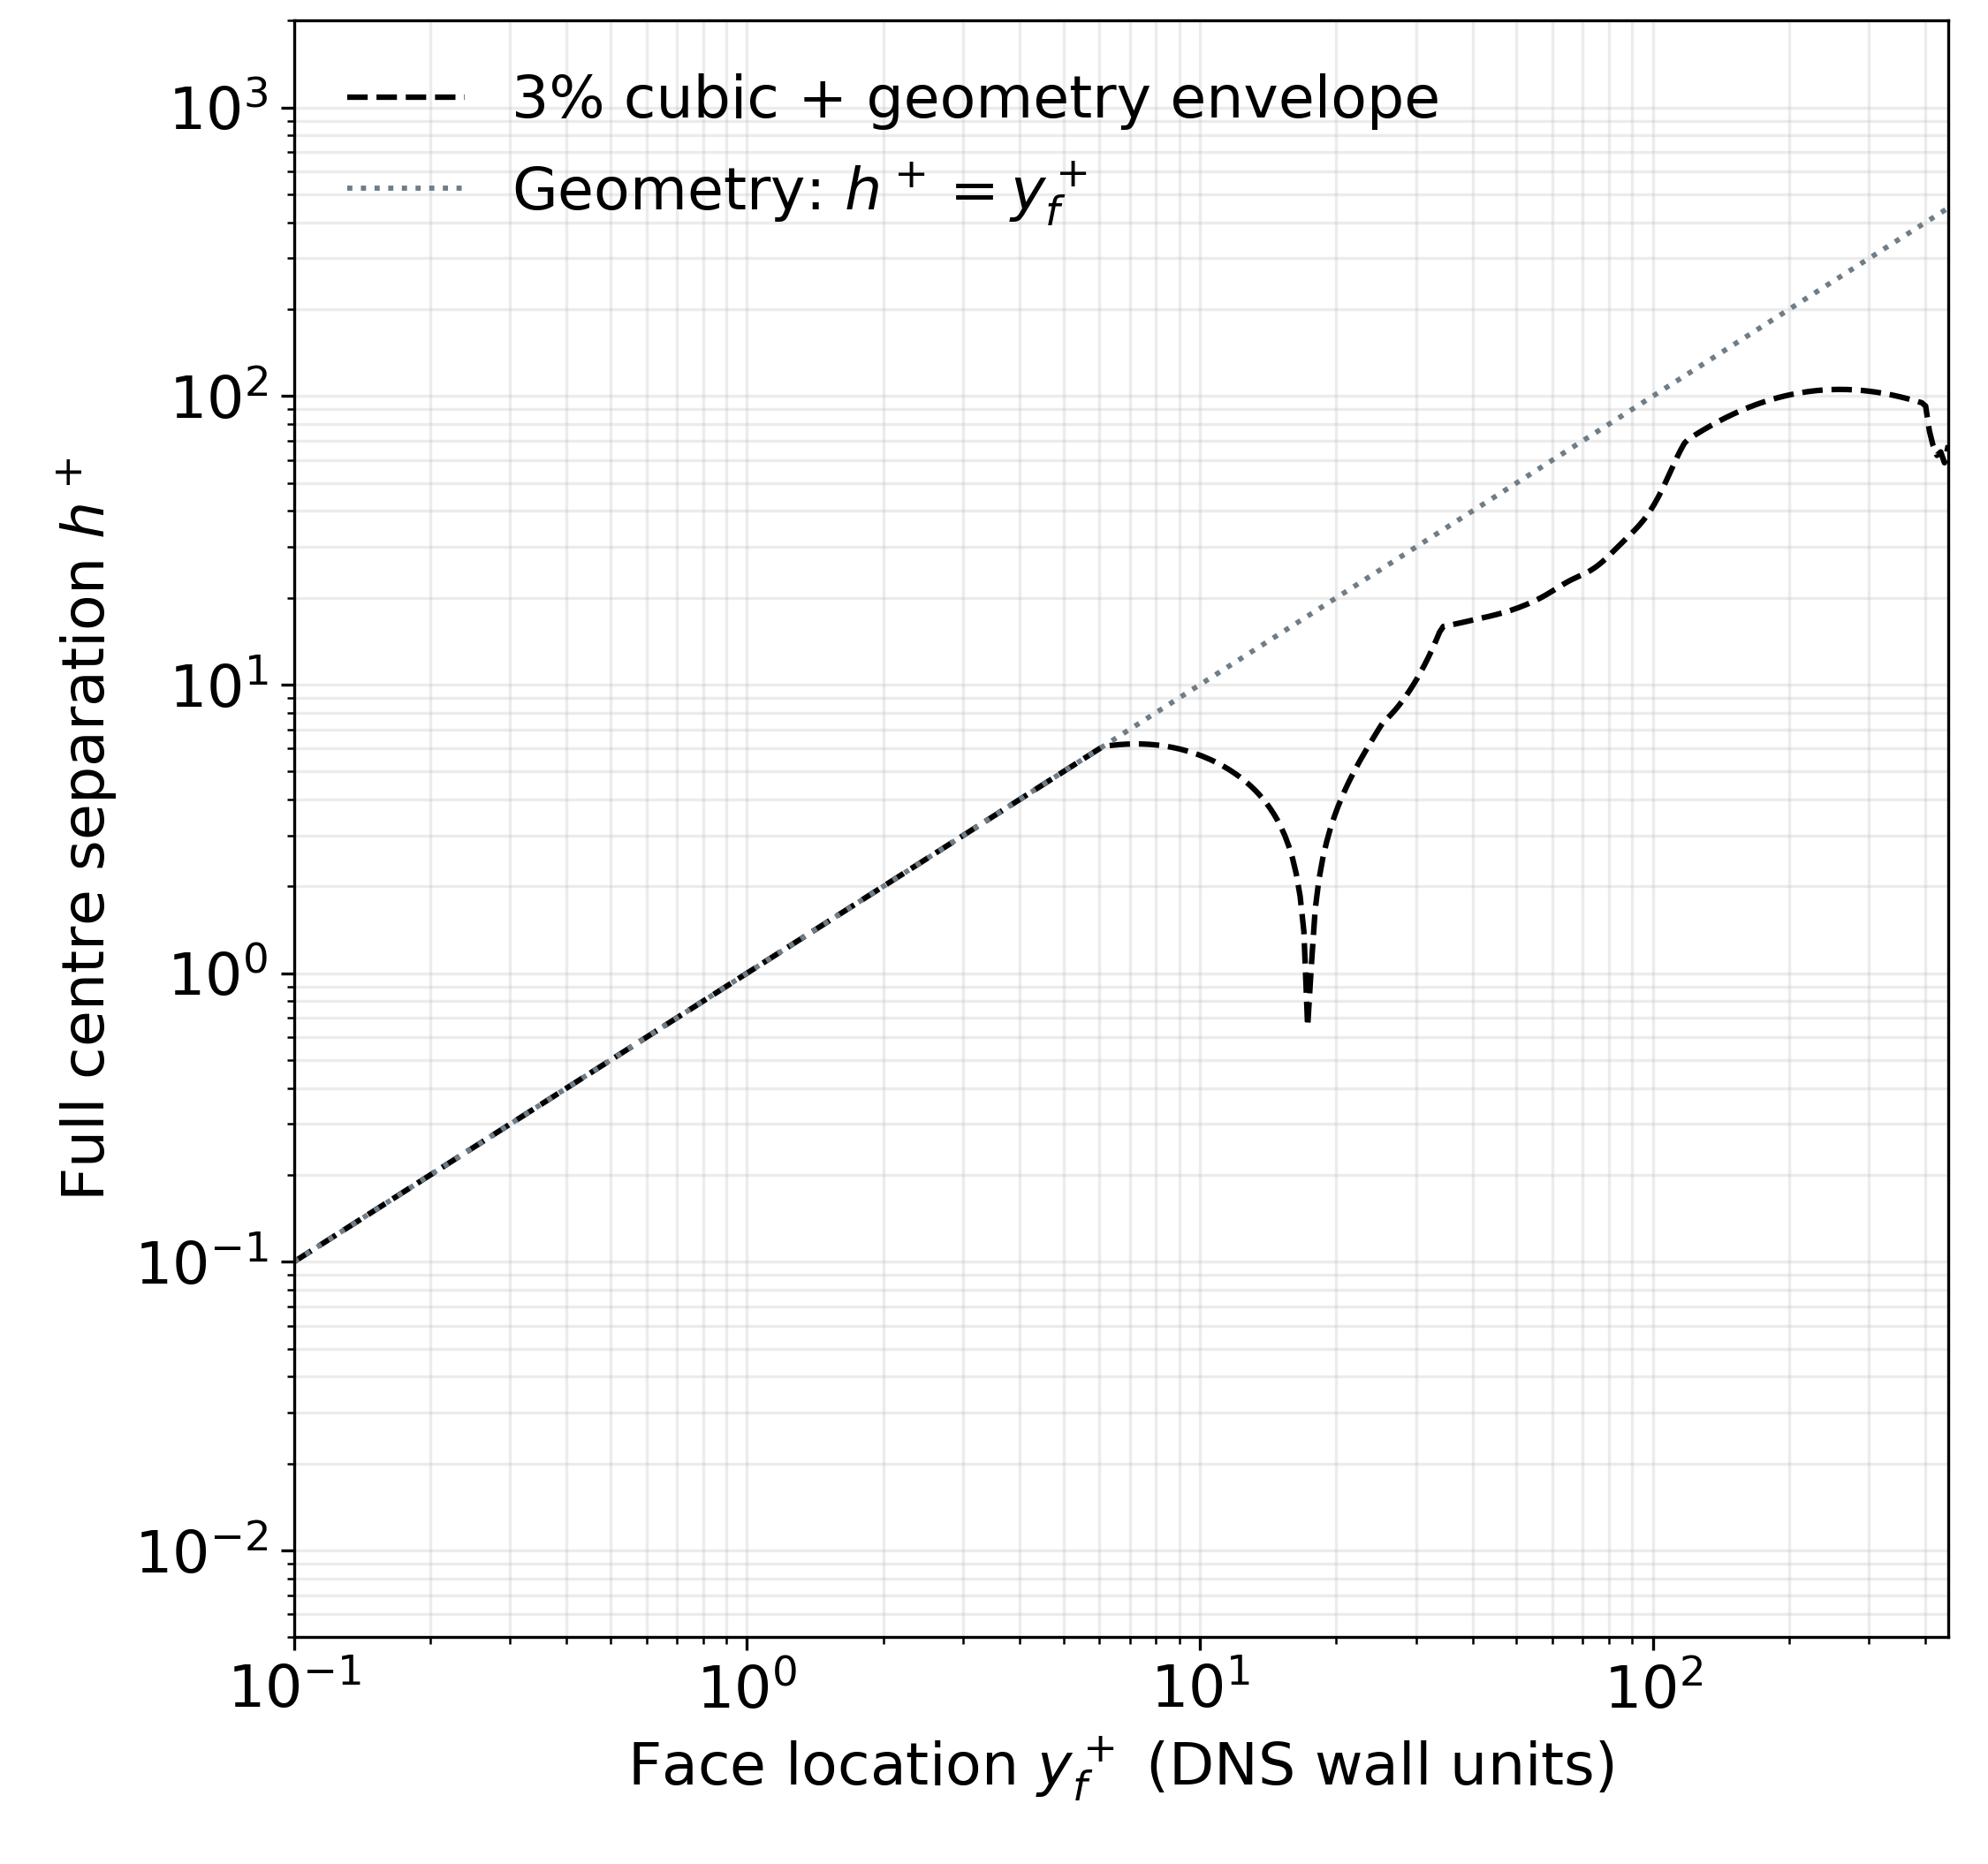
\includegraphics[width=0.7\linewidth,height=.62\textheight,keepaspectratio]{07_Error_Isolation_Results/Figures/WallFunctions/M6Tw025_3pct_envelope.png}
    \caption{Combined M6Tw025 spacing envelope for a $3\%$ component-error tolerance: the minimum of the four cubic-reference limits in Figure~\ref{fig:WF:M6Tw025-3pct-envelope-all-quantities}, profile support and the geometric cap $h^+=y_f^+$. The restrictive region near the temperature maximum requires substantially smaller centre separation than a conventional coarse stencil.}
    \label{fig:WF:M6Tw025-3pct-envelope-combined}
\end{figure}

Repeating the same analysis with $\epsilon=0.10$ gives Figure~\ref{fig:WF:M6Tw025-10pct-envelope-combined}. The restrictive minimum persists in the buffer region, whereas substantially larger spacings are admitted farther into the logarithmic region. Around $y_f^+\approx150$, the envelope reaches the geometric cap. Meaning a conventional symmetric coarse wall-function mesh stencil can locally satisfy the $10\%$ component tolerance and supports the finding discussed in Section~\ref{subsec:comparative:zpg:conventional-mesh}, that these log-layer regions are the ones used in the papers of Li et al. and Griffin et al. for validation purposes.

\begin{figure}[H]
    \centering
    % Figure provenance (WSL; absolute paths):
    %   Figure: /home/mgnadlinger/Xue_et_al/flat_plate/M6Tw025/opt_mesh/spacing_limits/M6Tw025_10pct_limits_only_font80.png
    %   Python scripts:
    %     /home/mgnadlinger/Xue_et_al/flat_plate/M6Tw025/opt_mesh/scripts/plot_cubic_limits_font80.py
    %     /home/mgnadlinger/Xue_et_al/flat_plate/M6Tw025/opt_mesh/scripts/plot_analysis.py
    %   Data / simulation roots (high-level):
    %     /home/mgnadlinger/Xue_et_al/flat_plate/M6Tw025/opt_mesh/spacing_limits
    %     /home/mgnadlinger/Xue_et_al/flat_plate/M6Tw025/opt_mesh/reference
    %     /home/mgnadlinger/Xue_et_al/flat_plate/M6Tw025/Digitizations
    %     /home/mgnadlinger/Xue_et_al/flat_plate/M6Tw025/Li_SA/SA_Prt0p9_baseline
    %   Note: Combined envelope is plotted from the finite-stencil limit tables generated by plot_analysis.py.
    % End figure provenance.
    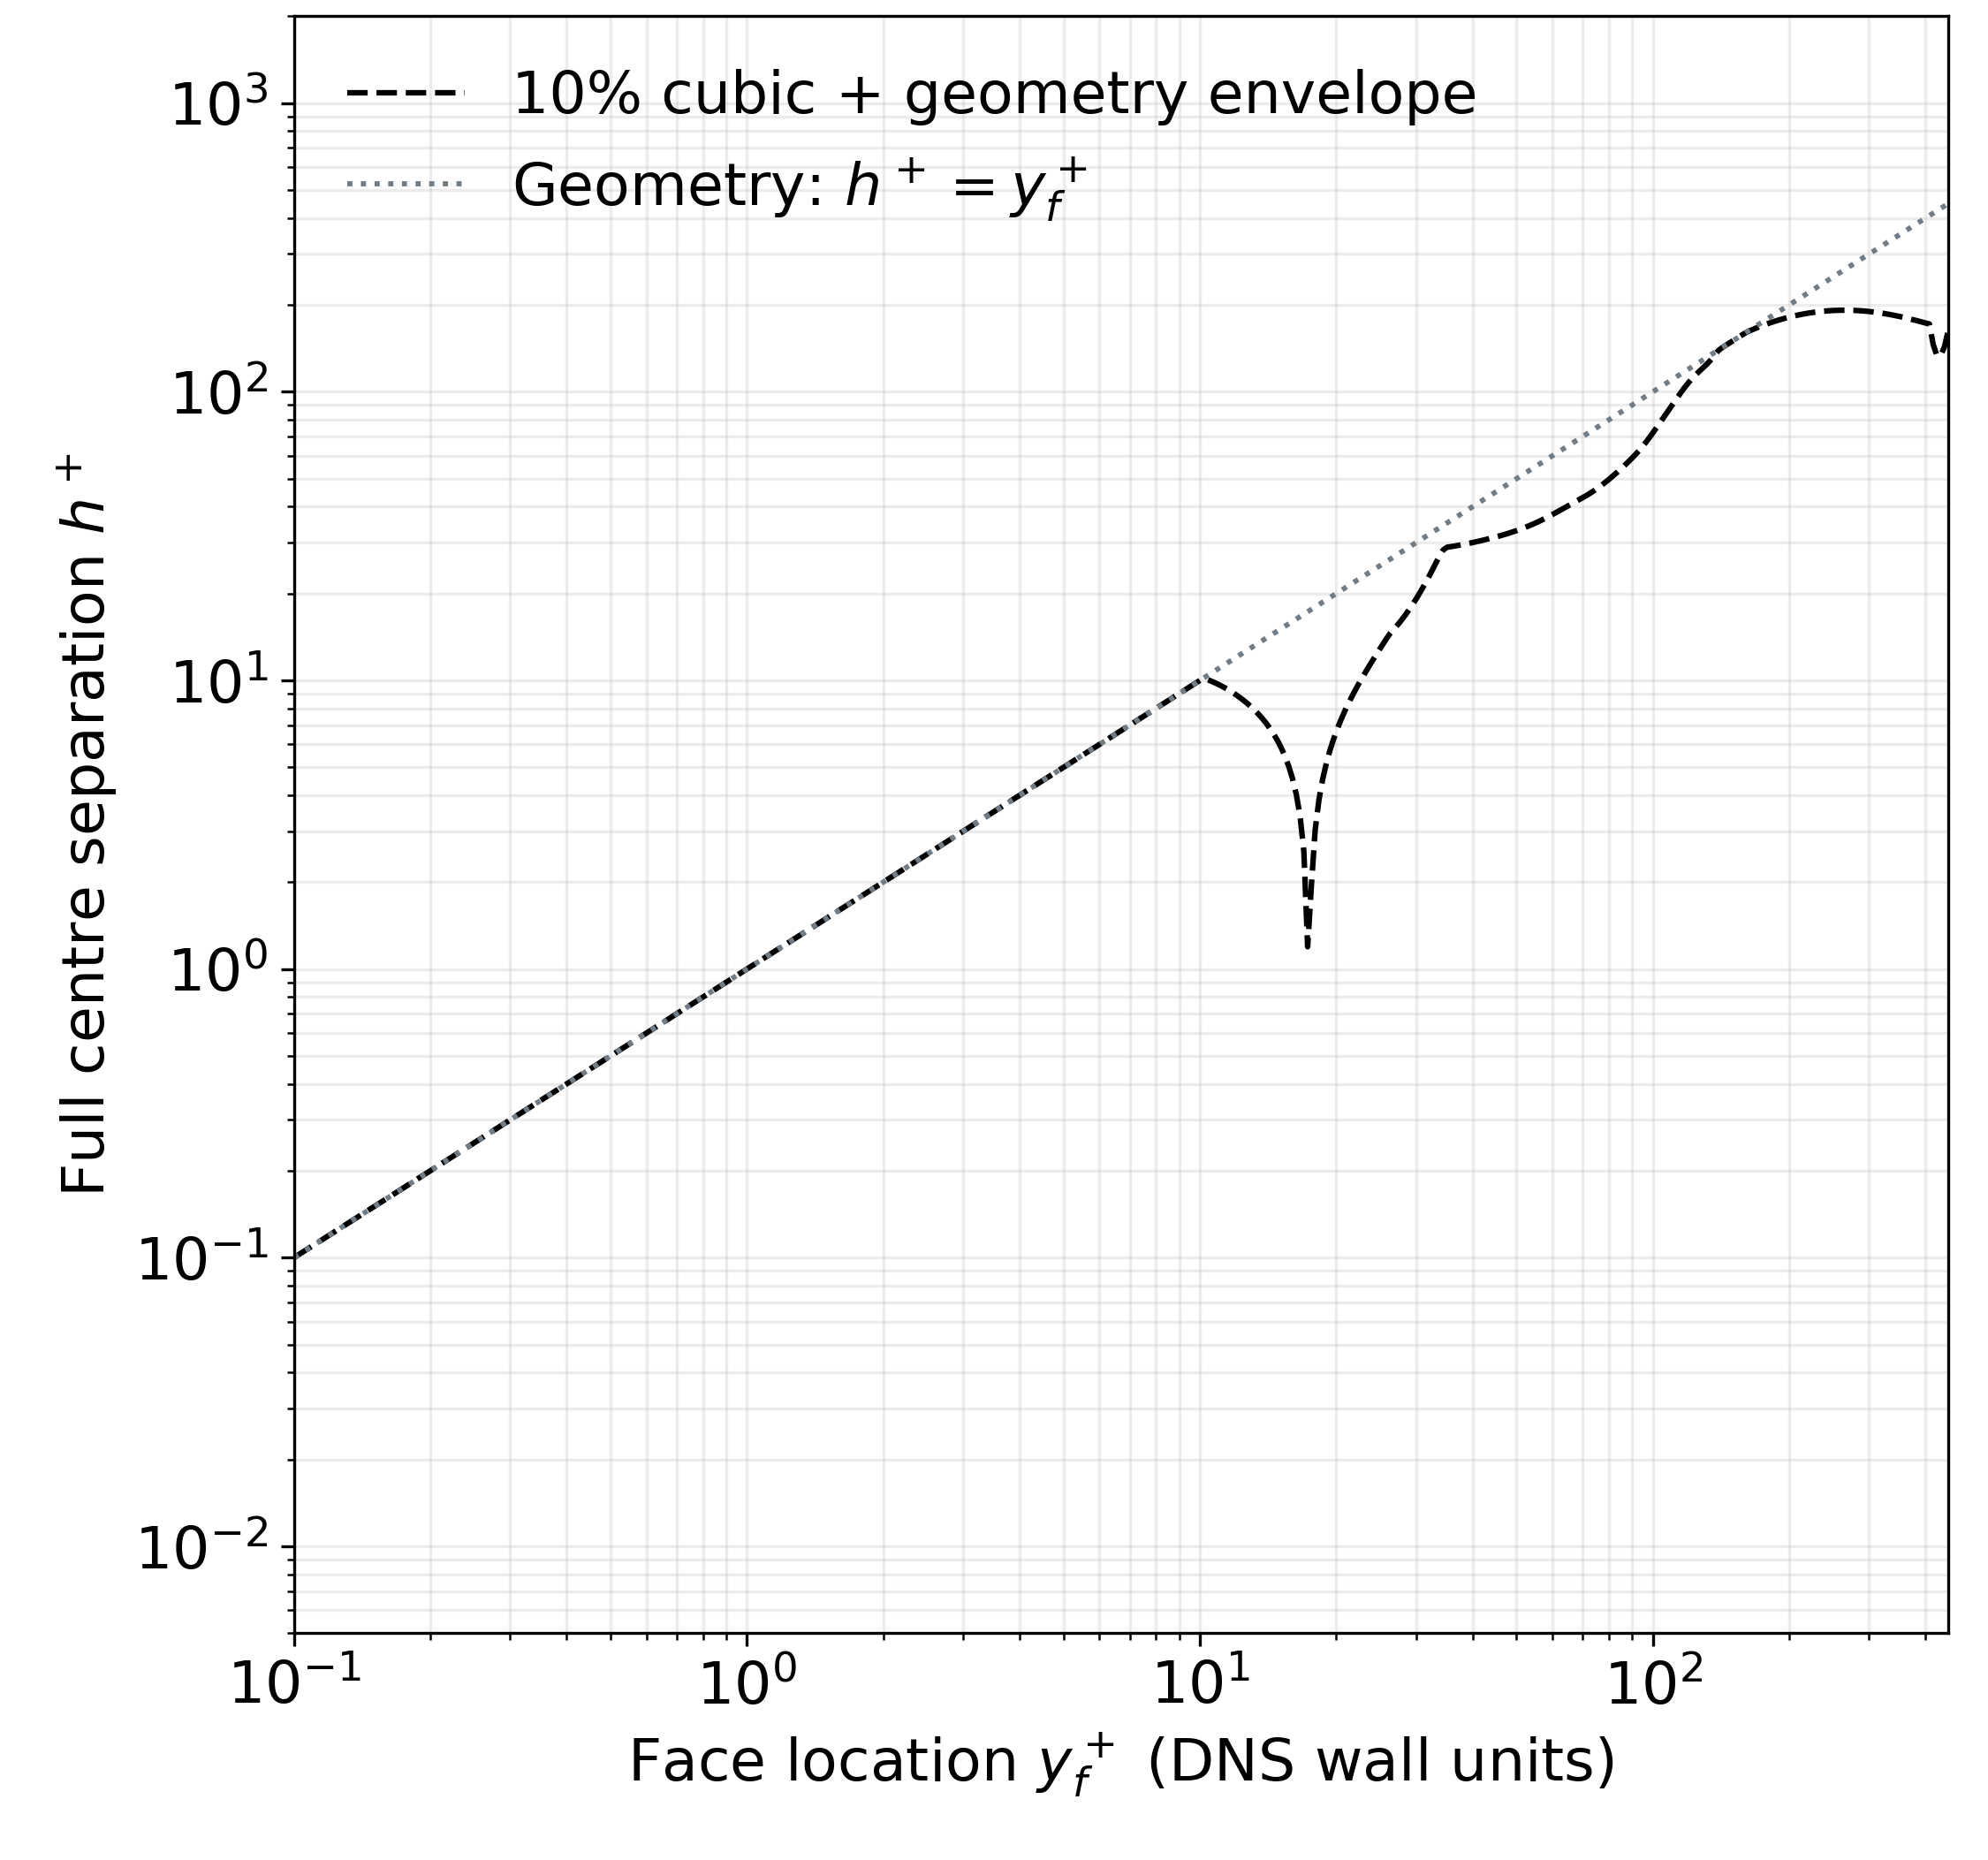
\includegraphics[width=0.7\linewidth,height=.62\textheight,keepaspectratio]{07_Error_Isolation_Results/Figures/WallFunctions/M6Tw025_10pct_envelope.png}
    \caption{Combined M6Tw025 spacing envelope with the local component-error tolerance relaxed to $10\%$. The restrictive minimum near the temperature maximum persists, while larger spacings are permitted farther outward. Around $y_f^+\approx150$, the envelope reaches the geometric cap and locally admits the conventional symmetric first-face stencil of Figure~\ref{fig:WF:exemplaray_y+10_mesh}. This is a local operator criterion, rather than a $10\%$ bound on CFD wall quantities.}
    \label{fig:WF:M6Tw025-10pct-envelope-combined}
\end{figure}

The physical reason on why this meshing restriction only arises now in hypersonic cold-wall boundary layers, and not in the subsonic or adiabatic-wall hypersonic cases can be seen in the comparative Figures~\ref{fig:WF:dns-velocity-profiles-linear} and~\ref{fig:WF:dns-temperature-profiles-linear}. There the M6Tw025 case is compared to the near-adiabatic M6Tw076 case and a transonic cold-wall case \textit{C09} of \cite{iwatani2025subharmonic}. Neither of the latter two cases show a pronounced temperature peak, and therefore the curvature variation is much less.

\begin{figure}[H]
    \centering
    % Figure provenance (paths relative to the thesis workspace root):
    % Original vector export: tmp/boundary_layer_profile_comparison/velocity_profiles_linear.pdf
    % Generating script: tmp/boundary_layer_profile_comparison/plot_linear_profiles.py
    % Shared data loading and styles: tmp/boundary_layer_profile_comparison/plot_profiles.py
    % Retained DNS files and preprocessing: tmp/boundary_layer_profile_comparison/raw/
    % Scaling checks and source URLs: tmp/boundary_layer_profile_comparison/source_notes.txt
    % Same DNS samples and normalizations as fig:background:dns-velocity-profiles:
    % Zhang, Duan and Choudhari (2018), DOI 10.2514/1.J057296;
    % Iwatani, Asada and Kawai (2025), DOI 10.1016/j.ijheatfluidflow.2025.109896.
    % C09: X=11, inferred velocity factor 0.8, conventional y+ reconstructed
    % from archived skin friction and wall properties, as documented in the background.
    % Linear y+ from 0 to 1200 includes all native samples and the wall points.
    % Copied without cropping or resizing the source PDF.
    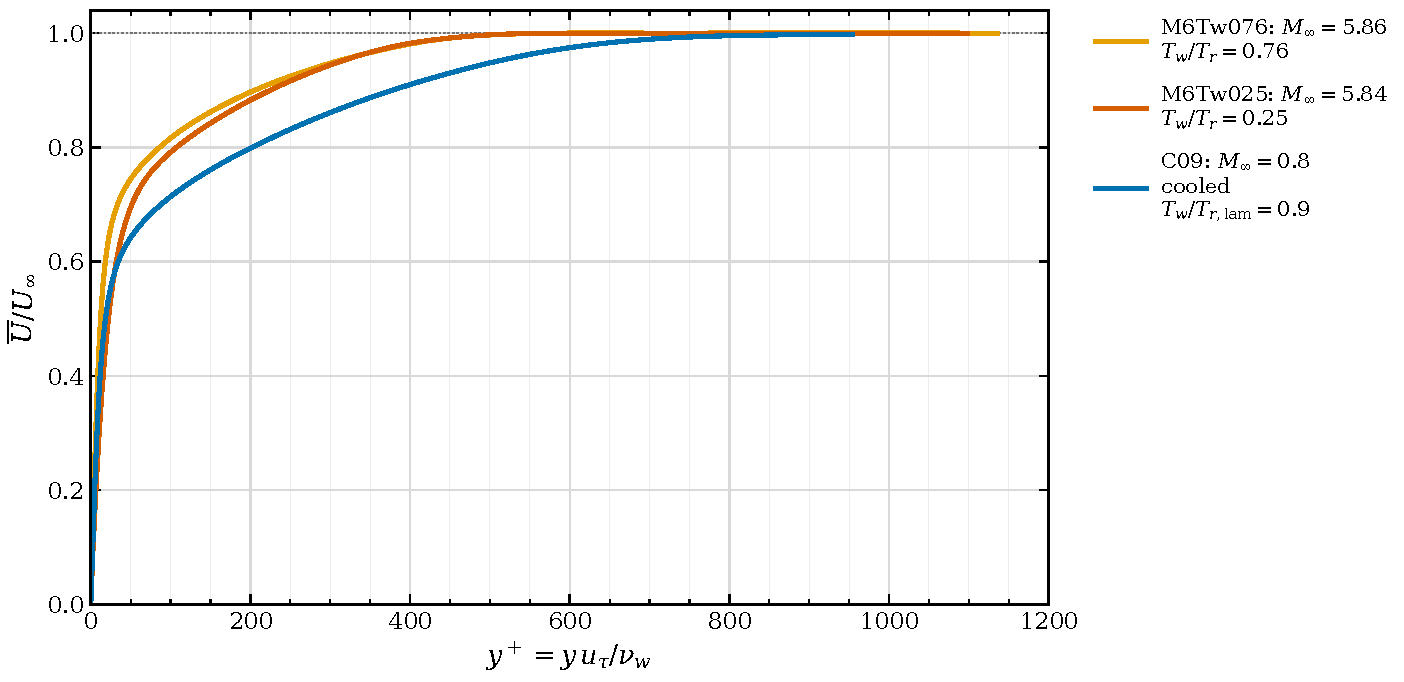
\includegraphics[width=\linewidth]{07_Error_Isolation_Results/Figures/Recon/velocity_profiles_linear.pdf}
    \caption[DNS velocity profiles on a linear wall-normal coordinate]{Freestream-normalized DNS velocity profiles for M6Tw076, M6Tw025 and C09, using the same data and normalization as Figure~\ref{fig:background:dns-velocity-profiles}, now plotted against linear \(y^+\). The native wall points at \(y^+=0\) are included.}
    \label{fig:WF:dns-velocity-profiles-linear}
\end{figure}

\begin{figure}[H]
    \centering
    % Figure provenance (paths relative to the thesis workspace root):
    % Original vector export: tmp/boundary_layer_profile_comparison/temperature_profiles_linear.pdf
    % Generating scripts, retained source data and scaling conventions:
    % as for fig:WF:dns-velocity-profiles-linear immediately above.
    % Native Reynolds-mean T/Tinf values are retained for all three cases.
    % Same thermal profiles as fig:background:dns-temperature-profiles;
    % linear y+ from 0 to 1200, including the native wall points, also in the C09 inset.
    % Copied without cropping or resizing the source PDF.
    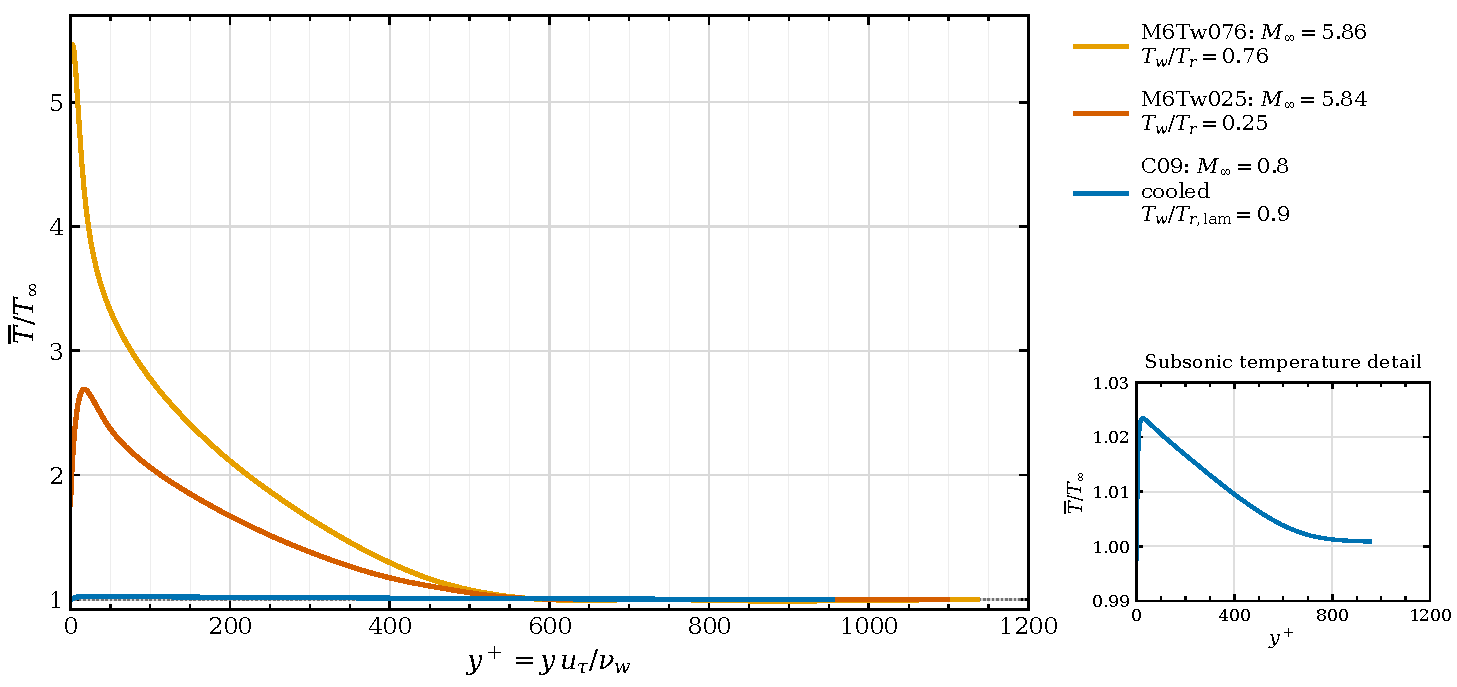
\includegraphics[width=\linewidth]{07_Error_Isolation_Results/Figures/Recon/temperature_profiles_linear.pdf}
    \caption[Linear thermal profiles and curvature variation near the cold-wall peak]{DNS temperature profiles from Figure~\ref{fig:background:dns-temperature-profiles}, shown on a linear \(y^+\) axis to better visualize the pronounced change in curvature associated with the hypersonic cold-wall M6Tw025 temperature peak. Since \(y^+\) is proportional to physical \(y\) within each case, this view connects the thermal-profile structure to finite stencil spacing and the reconstruction error illustrated by the secant--tangent comparison in Figure~\ref{fig:WF:exemplaray_y+10_reconstruction_error}. The C09 inset uses a separate vertical scale.}
    \label{fig:WF:dns-temperature-profiles-linear}
\end{figure}

All in all, the above analysis shows that the conventional coarse wall-function mesh stencil, paired with second-order accurate schemes, is not sufficient to resolve the internal-face transport in hypersonic cold-wall boundary layers. The pronounced temperature peak causes a large change in curvature, which in turn requires a much smaller centre separation than the conventional coarse wall-function mesh stencil provides. This novel mesh requirement is thus only dependant on the boundary layer profile and numerical schemes, in turn this requirement also applies to wall-resolved runs. In other words, the wall-functions can be understood as just a different heat-flux and shear stress relation than the convential linear correlation between the first off-wall cell cetner to the wall, as described for wall-resolved RANS in Equation~\eqref{eq:q_w_openFOAM_math}. But with the very low first-cell requirement of these wall-resolved runs on hypersonic cold-walls (i.e. the first-cell acoustic Reynolds number must be below 1 as discussed in Section~\ref{sec:evaluation:mesh-families-yplus}), only very extreme growth rates of the boundary layer mesh may run into any appreciable internal-face transport error, thus it remained undiscussed so far.
\par\medskip

The following section will show how proof this hypothesis by isolating these discretization errors through constructing boundary layer-informed meshes that satisfy the above discussed $3\%$ criterion.

\subsection{Wall functions on boundary layer-informed meshes}
\label{subsec:comparative:zpg:informed-mesh}

To test the above discussed error due to spatial discretization in CFD, families of boundary layer-informed meshes are constructed for prescribed wall-function sampling positions. This allows the wall-function sample to be swept over the whole $y^+$ range similar to the wall-closures a-priori analysis in Section~\ref{subsec:erriso:apriori-solver} and conventional mesh CFD runs in Figures~\ref{fig:WF:Li-LowHM3_conventional_mesh}--\ref{fig:WF:Griffin-M6Tw025_conventional_mesh}, while the internal-face spacing is controlled by the above discussed $3\%$ criterion. This arrangement reduces the coupling between moving the wall-function sample and the boundary layer spatial discretization.
\par\medskip

Figures~\ref{fig:WF:LowHM3-3pct-mesh-sweep} and~\ref{fig:WF:M6Tw025-3pct-mesh-sweep} show the resulting families for the M6Tw025 and LowH\_M3 case respectivly. The dotted and dashed lines are taken and constructed as described in the boundary layer analysis Section~\ref{subsec:comparative:zpg:mesh-criterion} above - specifically for the M6Two025 case, the Figure~\ref{fig:WF:M6Tw025-3pct-mesh-sweep} dashed and dotted lines are the same as in the Figure~\ref{fig:WF:M6Tw025-3pct-envelope-combined}. For the construction of the mesh families (see Figures~\ref{fig:WF:LowHM3-3pct-mesh-sweep} and~\ref{fig:WF:M6Tw025-3pct-mesh-sweep} right plots), a desired wall-function sampling height is prescribed and the internal-face spacing around it is then grown up until the allowable  discretization error of e.g. $3\%$ against the known profile is reached. This is continued until the whole boundary layer is covered. The resulting meshes are not a bound on the total CFD error or a proof of a globally optimal meshing, but aim to provide an isolation from this error source. The generated meshes are subsequently re-checked against the known boundary layer profiles, using their actual, generally unsymmetric, centre-to-face distances to ensure the desired spacing criterion is really satisfied.

\begin{figure}[H]
    \centering
    % Figure provenance (WSL; absolute paths):
    %   Figure: /home/mgnadlinger/WF_validation/LowH_M3/opt_meshes/marching_design/LowH_M3_mesh_sweep_3pct.png
    %   Python script:
    %     /home/mgnadlinger/WF_validation/LowH_M3/opt_meshes/marching_design/plot_mesh_report.py
    %   Data / simulation roots (high-level):
    %     /home/mgnadlinger/WF_validation/LowH_M3/opt_meshes/marching_design/3pct
    %     /home/mgnadlinger/WF_validation/LowH_M3/opt_meshes/marching_design/reference
    %     /home/mgnadlinger/WF_validation/LowH_M3/opt_meshes/Li_fitted_3pct_minCells_SA
    %     /home/mgnadlinger/WF_validation/LowH_M3/wall_resolved/SA/LowH_M3
    %   Note: Mesh-design report uses the frozen wall-resolved SA reference and the written fitted-Li mesh
    %     family.
    % End figure provenance.
    %   Print-size typography: regenerated at 170 mm width with 10 pt text; exact source data
    %     and local plotting script retained in Figures/WallFunctions/mesh_sweep_font_sources/.
    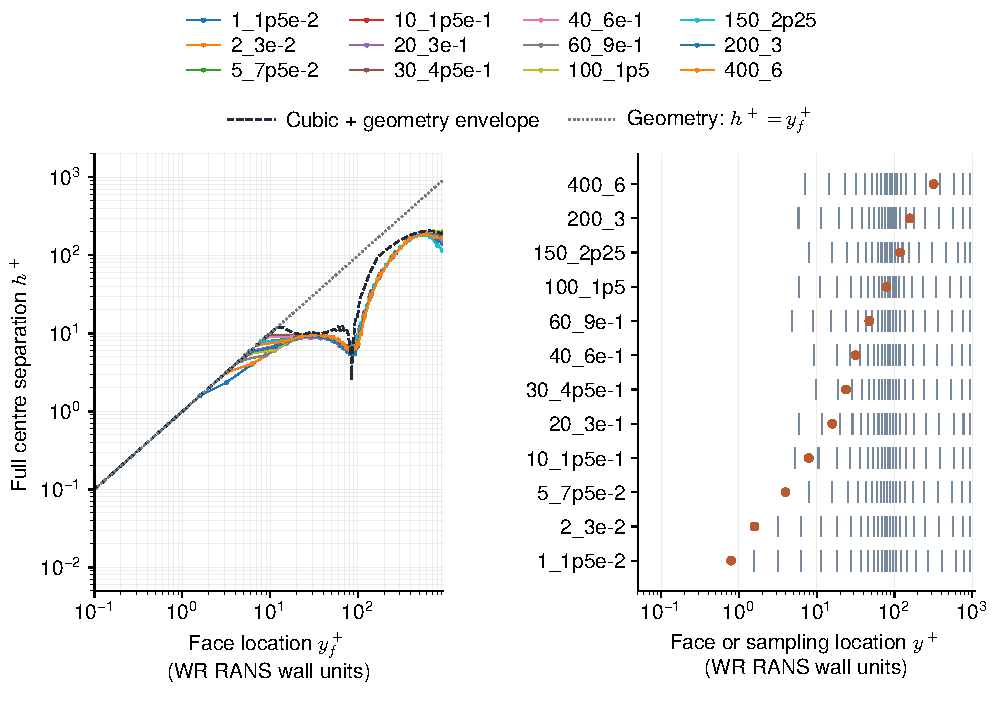
\includegraphics[width=\linewidth]{07_Error_Isolation_Results/Figures/WallFunctions/LowHM3_mesh_sweep_3pct.pdf}
    \caption{Boundary layer-informed $3\%$ spatial discretization error mesh family for LowH\_M3. The naming of the mesh families follows the structure \textit{desired wall-function sampling point in $y^+$}\_\textit{desired wall-function sampling point in millimetres}. Left: Black dotted and dashed lines represent the envelope stemming from the boundary layer analysis as described in Section~\ref{subsec:comparative:zpg:mesh-criterion}. The colourfull lines show the new boundary layer-informed meshes' actual spatial discretization error against the known boundary layer profiles, with all of them consistently staying below the $3\%$ envelope. Right: The actual mesh design (blue lines represent the position of the cell faces) and wall-function sampling centres (orange) are shown, with the pronounced clustering around the $y^+\approx85$ where the temperature peak sits for this case.} 
    \label{fig:WF:LowHM3-3pct-mesh-sweep}
\end{figure}

\begin{figure}[H]
    \centering
    % Figure provenance (WSL; absolute paths):
    %   Figure: /home/mgnadlinger/Xue_et_al/flat_plate/M6Tw025/opt_mesh/spacing_limits/M6Tw025_mesh_sweep_3pct.png
    %   Python script:
    %     /home/mgnadlinger/Xue_et_al/flat_plate/M6Tw025/opt_mesh/scripts/plot_analysis.py
    %   Data / simulation roots (high-level):
    %     /home/mgnadlinger/Xue_et_al/flat_plate/M6Tw025/opt_mesh/searches/3pct
    %     /home/mgnadlinger/Xue_et_al/flat_plate/M6Tw025/opt_mesh/Li_3pct_SA
    %     /home/mgnadlinger/Xue_et_al/flat_plate/M6Tw025/opt_mesh/spacing_limits
    %     /home/mgnadlinger/Xue_et_al/flat_plate/M6Tw025/opt_mesh/reference
    %     /home/mgnadlinger/Xue_et_al/flat_plate/M6Tw025/Digitizations
    %     /home/mgnadlinger/Xue_et_al/flat_plate/M6Tw025/Li_SA/SA_Prt0p9_baseline
    %   Note: Source report identifies this as the ordinary-Li mesh family.
    % End figure provenance.
    %   Print-size typography: regenerated at 170 mm width with 10 pt text; exact source data
    %     and local plotting script retained in Figures/WallFunctions/mesh_sweep_font_sources/.
    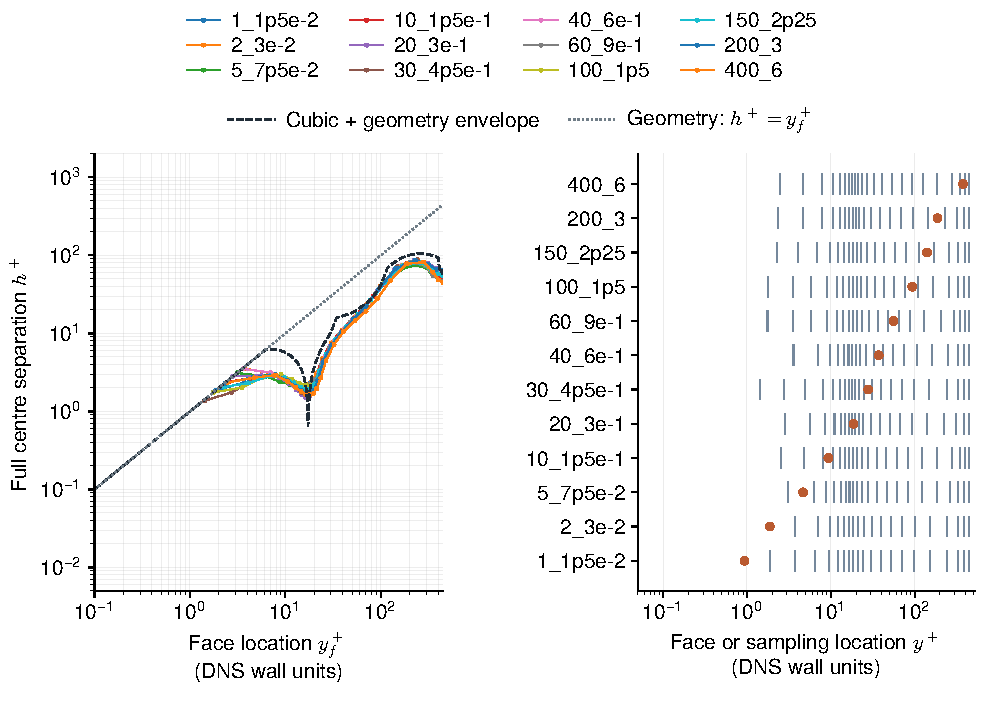
\includegraphics[width=\linewidth]{07_Error_Isolation_Results/Figures/WallFunctions/M6Tw025_mesh_sweep_3pct.pdf}
    \caption{Boundary layer-informed $3\%$ spatial discretization error mesh family for M6Tw025. The naming of the mesh families follows the structure \textit{desired wall-function sampling point in $y^+$}\_\textit{desired wall-function sampling point in millimetres}. Left: Black dotted and dashed lines represent the envelope stemming from the boundary layer analysis as described in Section~\ref{subsec:comparative:zpg:mesh-criterion}. The colourfull lines show the new boundary layer-informed meshes' actual spatial discretization error against the known boundary layer profiles, with all of them consistently staying below the $3\%$ envelope. Right: The actual mesh design (blue lines represent the position of the cell faces) and wall-function sampling centres (orange) are shown, with the pronounced clustering around the $y^+\approx18$ where the temperature peak sits for this case.}
    \label{fig:WF:M6Tw025-3pct-mesh-sweep}
\end{figure}

Figure~\ref{fig:WF:3pct-bl-informed-mesh-CFD-results} presents the CFD sweeps on these meshes. The abscissa is now the wall-function's sample location $y_s^+$, rather than necessarily the physical first-cell $y_1^+$. The reader is encouraged to look at the a-priori analysis, conventional coarase wall-function mesh CFD and herein presented boundary layer-informed mesh CFD results side by side for the four investigated combionations of Li wall function and Griffin wall function on the LowH\_M3 and M6Tw025 case (e.g. for the Li wall function on the LowH\_M3 case, see Figures~\ref{fig:wall-closure:a-priori-Li-LowHM3},~\ref{fig:WF:Li-LowHM3_conventional_mesh} and~\ref{fig:WF:3pct-bl-informed-mesh-CFD-results} top).
\par\medskip

It is immediatly apparant that the boundary layer-informed meshes follow the general error trend of the a-priori found closure error, significantly better than the conventional coarse wall-function meshes. The pronounced overshoot in the buffer layer that the conventional mesh exhibits in Figure~\ref{fig:WF:Li-LowHM3_conventional_mesh} is removed and the boundary layer-informed meshes in Figure~\ref{fig:WF:3pct-bl-informed-mesh-CFD-results} (top) show significantly closer trend to the a-priori results of Figure~\ref{fig:wall-closure:a-priori-Li-LowHM3}. Also indicative is, that Figure~\ref{fig:WF:Li-LowHM3_conventional_mesh} from $y^+\approx2$ onwards deviated from the wall-resolved baseline, whereas the boundary layer-informed meshes in Figure~\ref{fig:WF:3pct-bl-informed-mesh-CFD-results} (top) follow the a-priori in Figure~\ref{fig:wall-closure:a-priori-Li-LowHM3}, of effectly zero error, up to the same $y^+\approx10$.
\par\medskip

Because of error addition and cancellation, the wall-function CFD results on the boundary layer-informed meshes do not exactly match the quantiataive errors of the a-priori analysis. Arguably an even finer boundary layer-informed mesh with $\epsilon_max \le 0.1\%$ could be designed to further isolate the discretization errors, this highlights how big of an impact even these small discretization errors can have. For comparing the M6Tw025 cases, one should also keep in mind, that an additonal uncertainty arises in the discovered fact, that the turbulence model is not capable to reproduce the DNS temperature peak, as discussed in Section~\ref{subsec:comparative:zpg:wr-profiles} and investigated implications in Section~\ref{subsec:erriso:rans-profile-influence}.
\par\medskip

The highest sampling positions require particular caution. The LowH\_M3 Li curve rises markedly at its outermost sample, where inner-layer and approximately constant-stress assumptions become less suitable as discussed in the a-prori analysis in Section~\ref{subsec:comparative:zpg:apriori-mesh}. This point does not establish a general acceptable upper $y_s^+$, since the relevant boundary layer region and the closure's usable range are case dependent.
\par\medskip

From the analysis there is a strong conclusion from the CFD results of the herin used boundary layer-informed meshes vs. the previous conventional meshes, that the large error in the buffer layer and lower log-layer is driven by the spatial discretization error discussed as hypthesized.

\begin{figure}[H]
    \centering
    % Figure provenance (WSL; absolute paths):
    %   Figure: /home/mgnadlinger/WF_validation/LowH_M3/validation/outputs/plots/opt_mesh/li_3pct_mincells_sa_dns_station_relative_error.png
    %   Python scripts:
    %     /home/mgnadlinger/WF_validation/LowH_M3/validation/scripts/plot_opt_mesh_wall_flux_sweeps.py
    %     /home/mgnadlinger/WF_validation/LowH_M3/validation/scripts/plot_wall_flux_sweeps.py
    %   Data / simulation roots (high-level):
    %     /home/mgnadlinger/WF_validation/LowH_M3/opt_meshes/Li_3pct_minCells_SA
    %     /home/mgnadlinger/WF_validation/LowH_M3/wall_resolved/SA/LowH_M3
    %     /home/mgnadlinger/WF_validation/LowH_M3/Digitizations
    %   Note: Thesis image removes the 128-pixel title strip from the source export.
    % End figure provenance.
    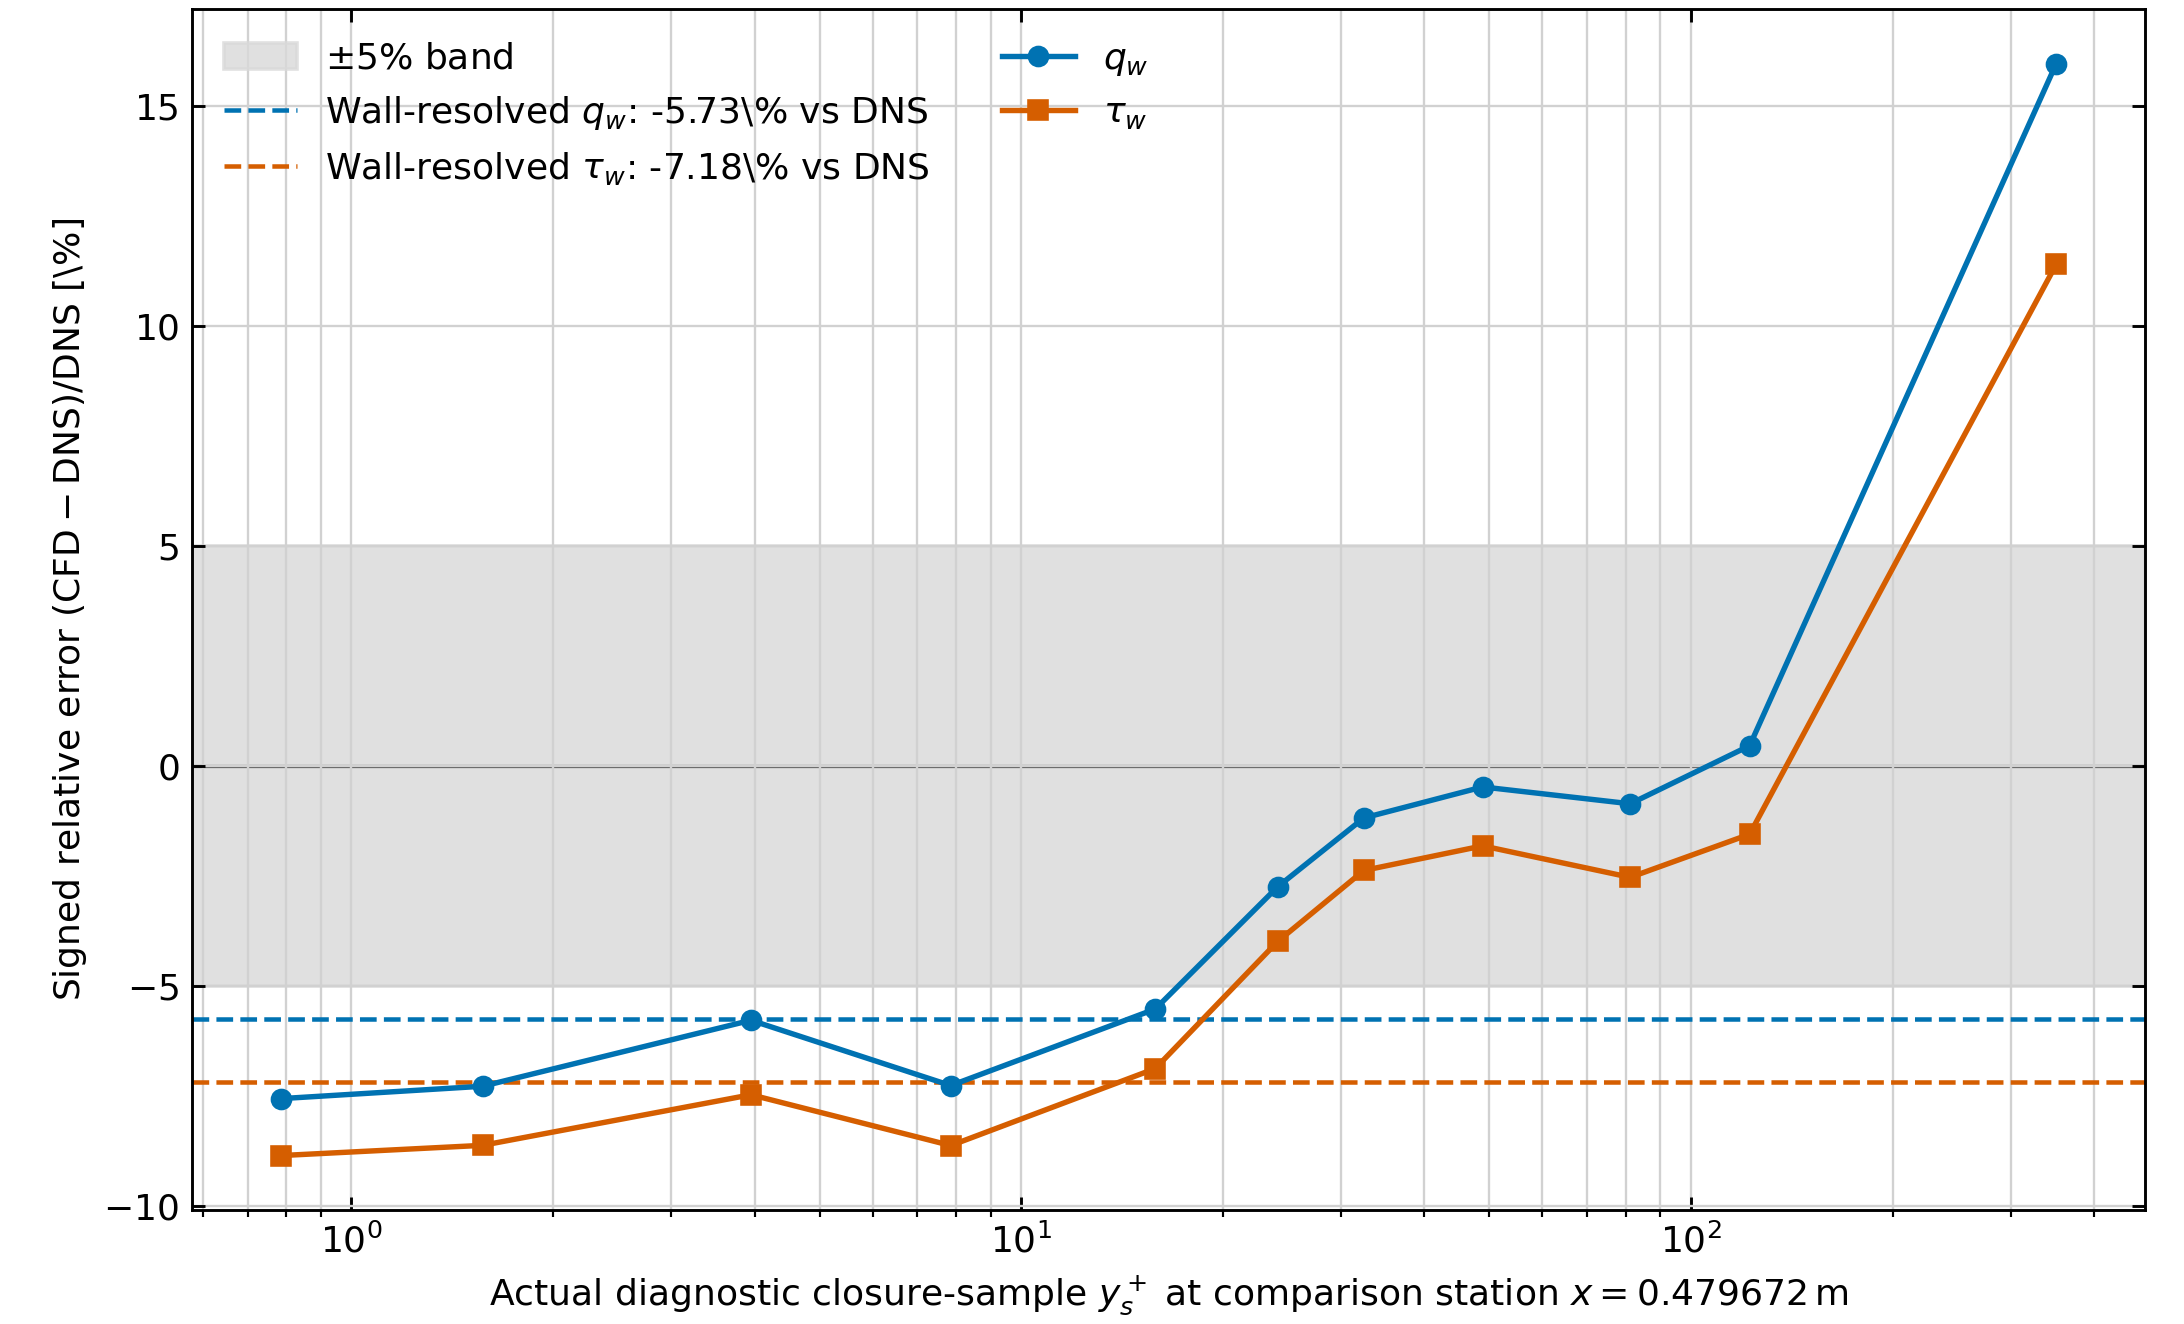
\includegraphics[width=\linewidth,height=.40\textheight,keepaspectratio]{07_Error_Isolation_Results/Figures/WallFunctions/04_3pctMesh_Li_LowHM3.png}
    % Figure provenance (WSL; absolute paths):
    %   Figure: /home/mgnadlinger/WF_validation/LowH_M3/validation/outputs/plots/opt_mesh/griffin_3pct_mincells_sa_dns_station_relative_error.png
    %   Python scripts:
    %     /home/mgnadlinger/WF_validation/LowH_M3/validation/scripts/plot_opt_mesh_wall_flux_sweeps.py
    %     /home/mgnadlinger/WF_validation/LowH_M3/validation/scripts/plot_wall_flux_sweeps.py
    %   Data / simulation roots (high-level):
    %     /home/mgnadlinger/WF_validation/LowH_M3/opt_meshes/Griffin_3pct_minCells_SA
    %     /home/mgnadlinger/WF_validation/LowH_M3/wall_resolved/SA/LowH_M3
    %     /home/mgnadlinger/WF_validation/LowH_M3/Digitizations
    % End figure provenance.
    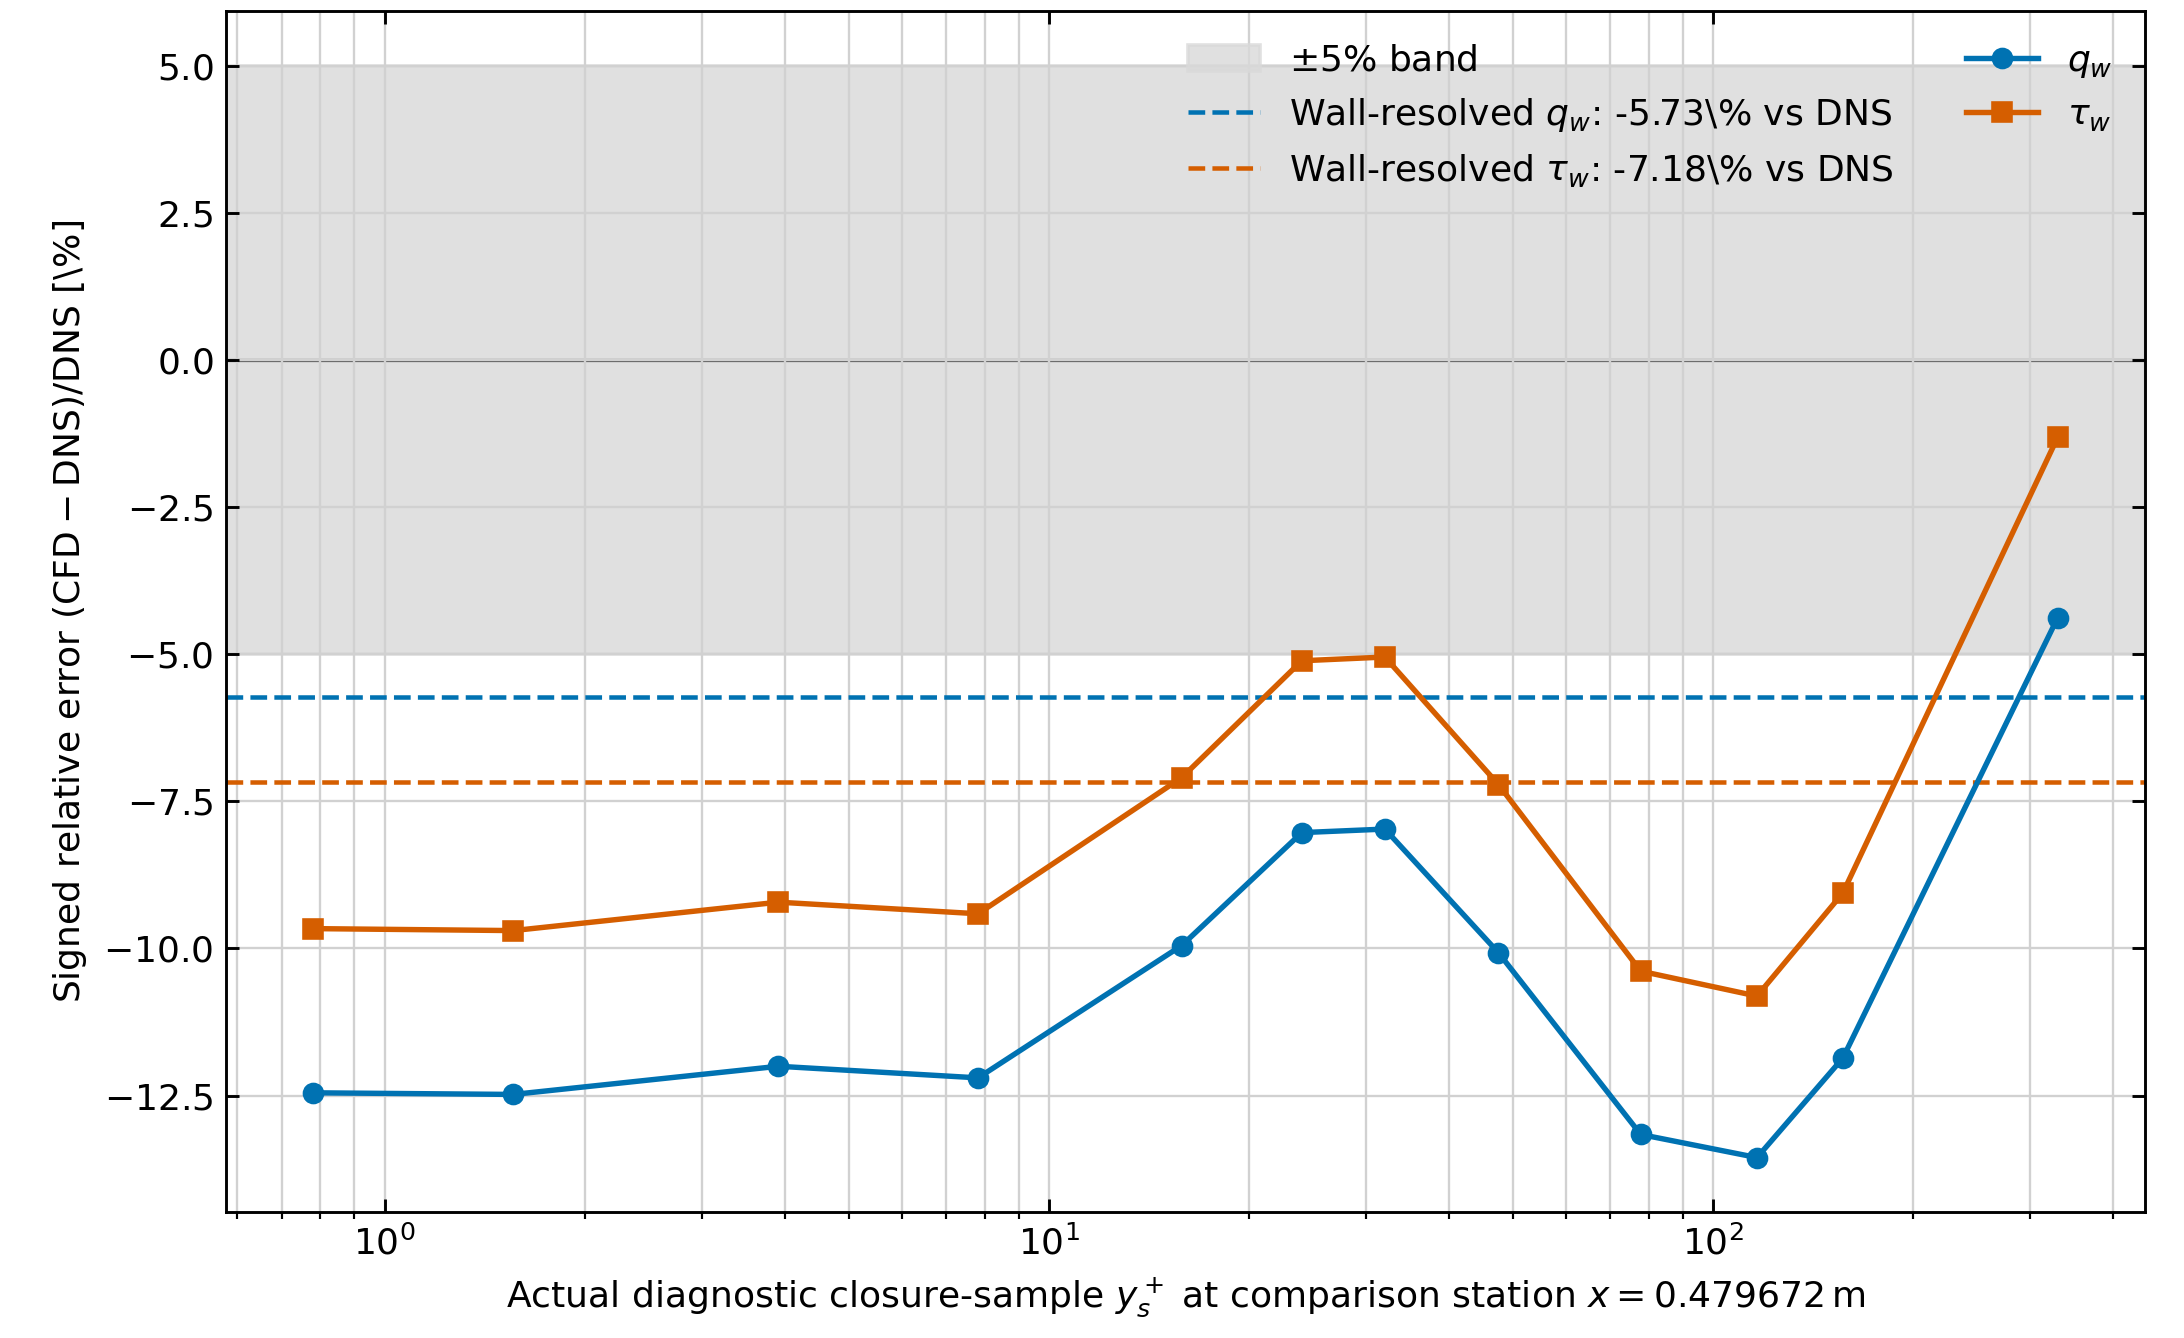
\includegraphics[width=\linewidth,height=.40\textheight,keepaspectratio]{07_Error_Isolation_Results/Figures/WallFunctions/04_3pctMesh_Griffin_LowHM3.png}
    \caption{Wall-function CFD on boundary layer-informed meshes designed with the $3\%$ cubic-reference component criterion. LowH\_M3 results are shown for Li (top) and Griffin (bottom). The abscissa is the actual diagnostic sampling location $y_s^+$ for the wall-function, not the first cell height. Dashed lines denote the wall-resolved baseline; shading marks $\pm5\%$ relative to DNS.}
    \label{fig:WF:3pct-bl-informed-mesh-CFD-results}
\end{figure}q

\begin{figure}[H]
    \ContinuedFloat
    \centering
    % Figure provenance (WSL; absolute paths):
    %   Figure: /home/mgnadlinger/Xue_et_al/flat_plate/M6Tw025/validation/outputs/plots/opt_mesh/li_3pct_sa_dns_station_relative_error.png
    %   Python scripts:
    %     /home/mgnadlinger/Xue_et_al/flat_plate/M6Tw025/validation/scripts/plot_opt_mesh_wall_flux_sweeps.py
    %     /home/mgnadlinger/Xue_et_al/flat_plate/M6Tw025/validation/scripts/plot_wall_flux_sweeps.py
    %   Data / simulation roots (high-level):
    %     /home/mgnadlinger/Xue_et_al/flat_plate/M6Tw025/opt_mesh/Li_3pct_SA
    %     /home/mgnadlinger/Xue_et_al/flat_plate/M6Tw025/Li_SA/SA_Prt0p9_baseline
    %     /home/mgnadlinger/Xue_et_al/flat_plate/M6Tw025/Digitizations
    %     /home/mgnadlinger/Xue_et_al/flat_plate/M6Tw025/opt_mesh/reference/sources
    % End figure provenance.
    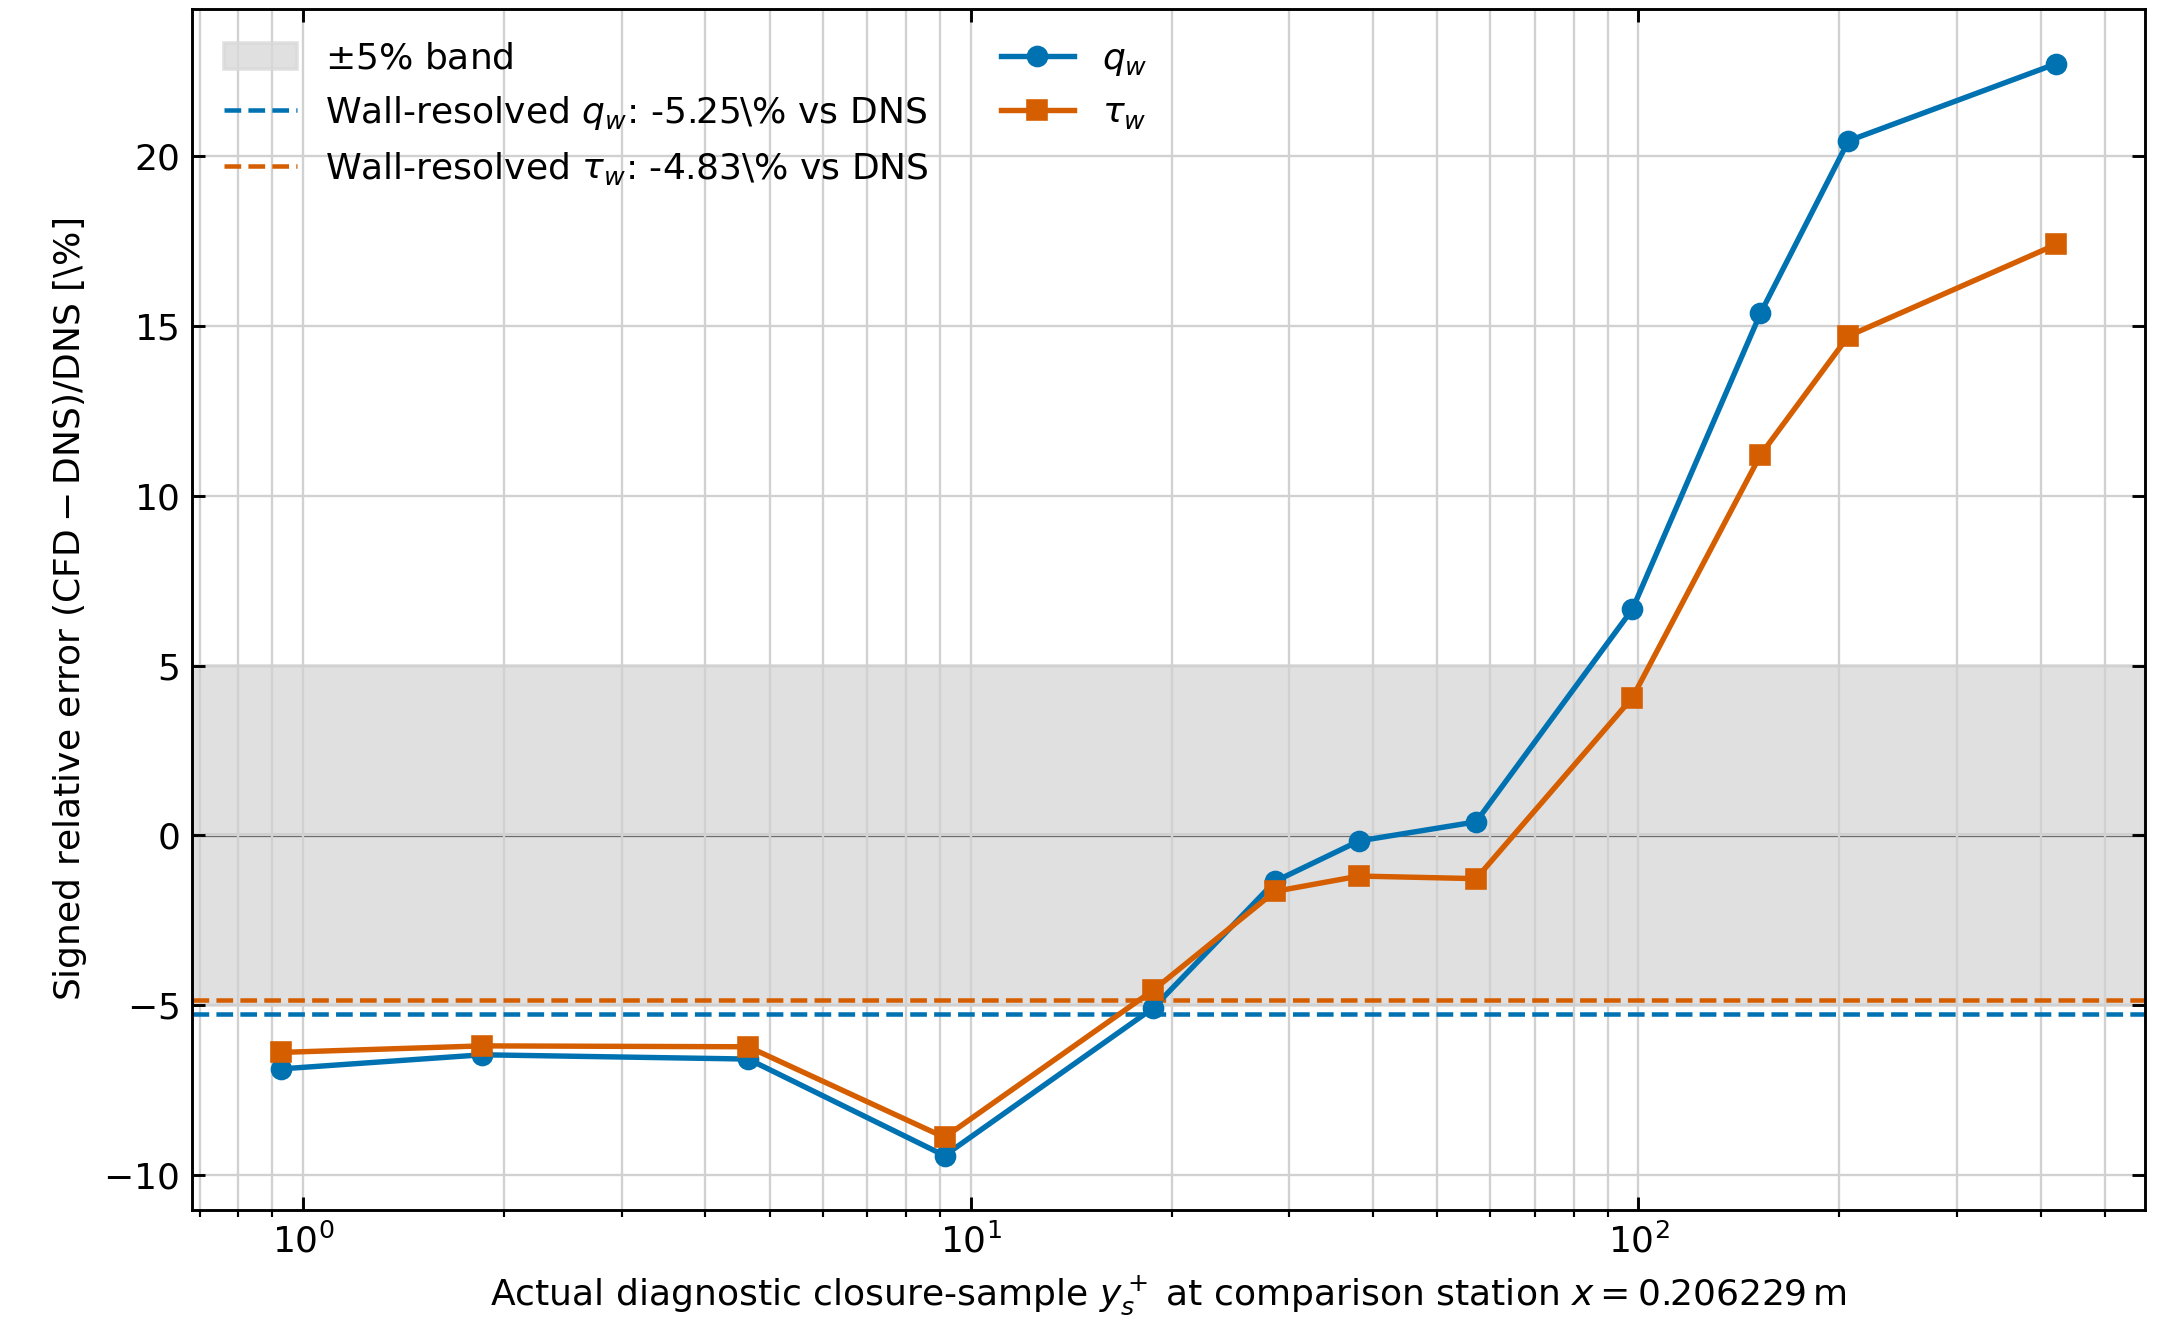
\includegraphics[width=\linewidth,height=.40\textheight,keepaspectratio]{07_Error_Isolation_Results/Figures/WallFunctions/04_3pctMesh_Li_M6Tw025.png}
    % Figure provenance (WSL; absolute paths):
    %   Figure: /home/mgnadlinger/Xue_et_al/flat_plate/M6Tw025/validation/outputs/plots/opt_mesh/griffin_3pct_sa_dns_station_relative_error.png
    %   Python scripts:
    %     /home/mgnadlinger/Xue_et_al/flat_plate/M6Tw025/validation/scripts/plot_opt_mesh_wall_flux_sweeps.py
    %     /home/mgnadlinger/Xue_et_al/flat_plate/M6Tw025/validation/scripts/plot_wall_flux_sweeps.py
    %   Data / simulation roots (high-level):
    %     /home/mgnadlinger/Xue_et_al/flat_plate/M6Tw025/opt_mesh/Griffin_3pct_SA
    %     /home/mgnadlinger/Xue_et_al/flat_plate/M6Tw025/Li_SA/SA_Prt0p9_baseline
    %     /home/mgnadlinger/Xue_et_al/flat_plate/M6Tw025/Digitizations
    %     /home/mgnadlinger/Xue_et_al/flat_plate/M6Tw025/opt_mesh/reference/sources
    % End figure provenance.
    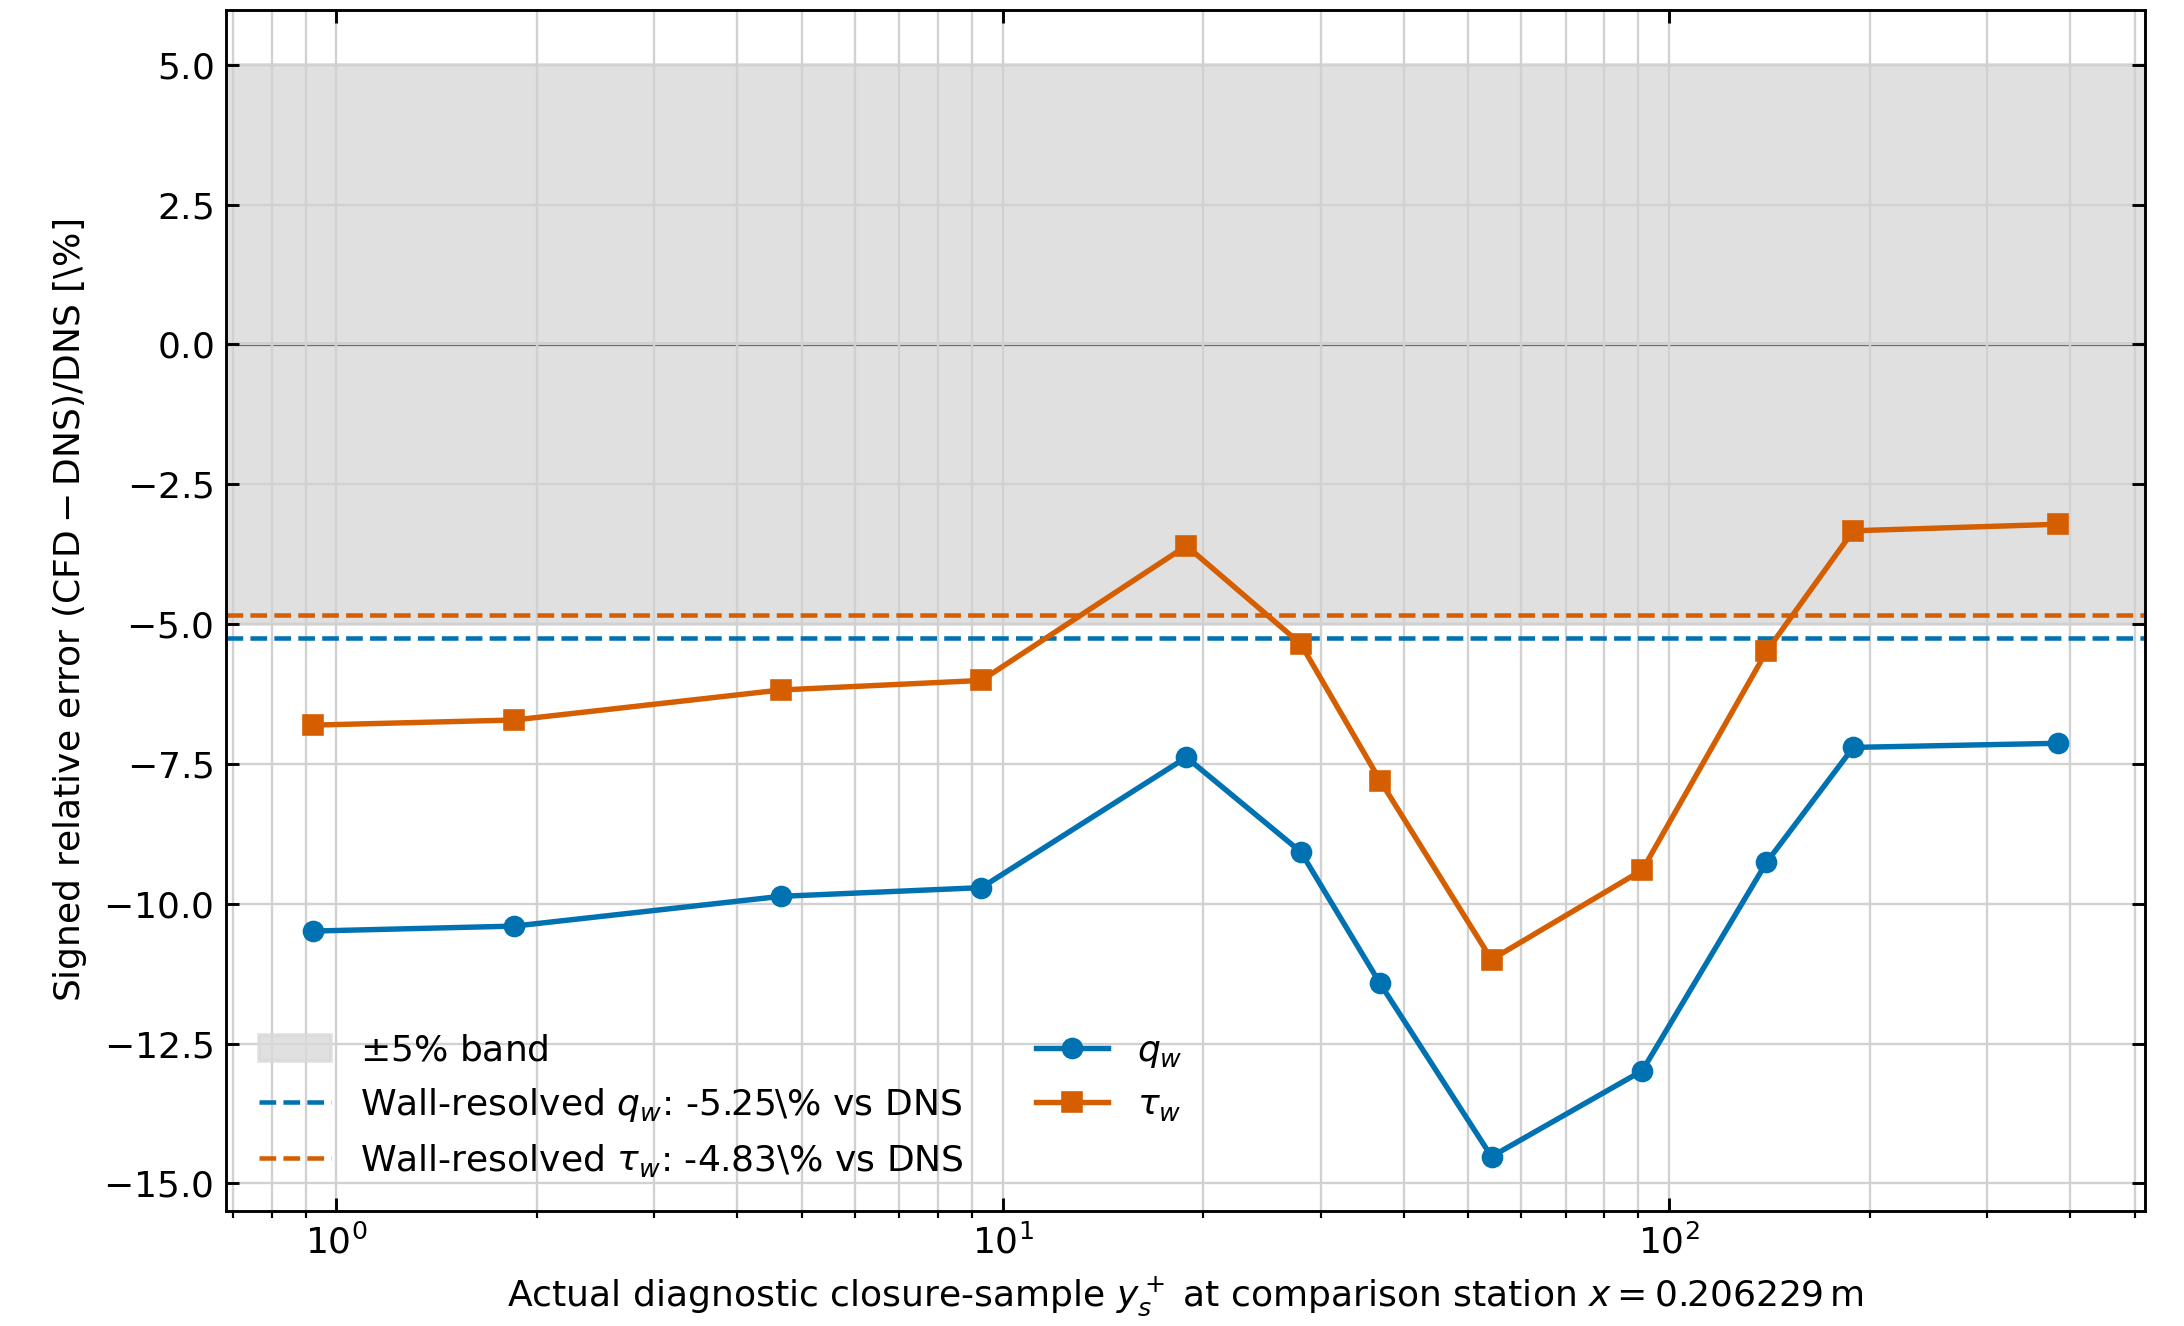
\includegraphics[width=\linewidth,height=.40\textheight,keepaspectratio]{07_Error_Isolation_Results/Figures/WallFunctions/04_3pctMesh_Griffin_M6Tw025.png}
    \caption[]{M6Tw025 results for Li (top) and Griffin (bottom), with SA and DNS normalization at $x=0.206229\,\mathrm{m}$. The mesh criterion and sampling-height definition are the same as in the preceding panels.}
\end{figure}

\subsection{Conditional a-priori estimation of the mesh requirement}
\label{subsec:comparative:zpg:apriori-mesh}

The above analysis and the novel proposed boundary layer informed meshing criterion, has one practical shortcoming: it requires knowledge of the resolved boundary layer profile. For an engineering approach, it is desirable to have a mesh design tool that does not require the resolved profile, but can still provide a-priori guidance on the required mesh spacing. The closures of the analytical Li et al. wall-function \cite{li2025WF} have this knowledge about hypersonic boundary layer backed in by design. Given wall shear and heat-flux, wall thermodynamic and transport properties, and an edge state, the wall-function closures can reconstruct the underlying profiles from which then the same finite-stencil limits can be evaluated. In the constant-$c_p$ form used here, the enthalpy relation supplies temperature from velocity, and the velocity law supplies the wall-normal coordinate. Under the additional constant-total-shear assumption, effective viscosity follows from $\mu_{\mathrm{eff}}=\tau_w/(\partial U/\partial y)$. Prescribed molecular and turbulent Prandtl numbers then give an effective conductivity estimate.
\par\medskip

Figure~\ref{fig:WF:a-priori-M6Tw025-10pct-envelope-combined} compares this estimate with the M6Tw025 profile-based envelope at a $10\%$ error tolerance. The reconstruction uses scalar DNS metadata for the wall loads and edge/wall states, without using the resolved profile values. It is therefore an assessment conditional on known loads, rather than an independent prediction of those loads. The broad inner-layer spacing trend is recovered, but the most restrictive minimum is shifted because the Li reconstruction places the temperature maximum closer to the wall. Near that maximum, even a modest position error can produce a large difference in the relative-gradient criterion. Differences toward the boundary layer edge also reflect the limited outer-layer representation of the reconstructed inner law.

\begin{figure}[H]
    \centering
    % Figure provenance (WSL; absolute paths):
    %   Figure: /home/mgnadlinger/Xue_et_al/flat_plate/M6Tw025/opt_mesh/li_apriori/M6Tw025_Li_combined_comparison_10pct_only.png
    %   Python scripts:
    %     /home/mgnadlinger/Xue_et_al/flat_plate/M6Tw025/opt_mesh/li_apriori/plot_10pct_combined_only.py
    %     /home/mgnadlinger/Xue_et_al/flat_plate/M6Tw025/opt_mesh/li_apriori/li_apriori_spacing.py
    %   Data / simulation roots (high-level):
    %     /home/mgnadlinger/Xue_et_al/flat_plate/M6Tw025/opt_mesh/li_apriori
    %     /home/mgnadlinger/Xue_et_al/flat_plate/M6Tw025/opt_mesh/spacing_limits
    %     /home/mgnadlinger/Xue_et_al/flat_plate/M6Tw025/opt_mesh/reference
    %     /home/mgnadlinger/Xue_et_al/flat_plate/M6Tw025/Digitizations
    %     /home/mgnadlinger/Xue_et_al/flat_plate/M6Tw025/Li_SA/SA_Prt0p9_baseline
    %   Note: Thesis image is cropped from the source export at native resolution, without resizing.
    %     Crop box in source pixels (left, top, right, bottom): (0, 274, 2250, 2200);
    %     resulting size: 2250 x 1926 pixels. Original plot proportions are preserved.
    %   Note: li_apriori_spacing.py generates the prediction from DNS scalar header inputs; the frozen DNS/SA
    %     reference supplies the comparison envelope.
    % End figure provenance.
    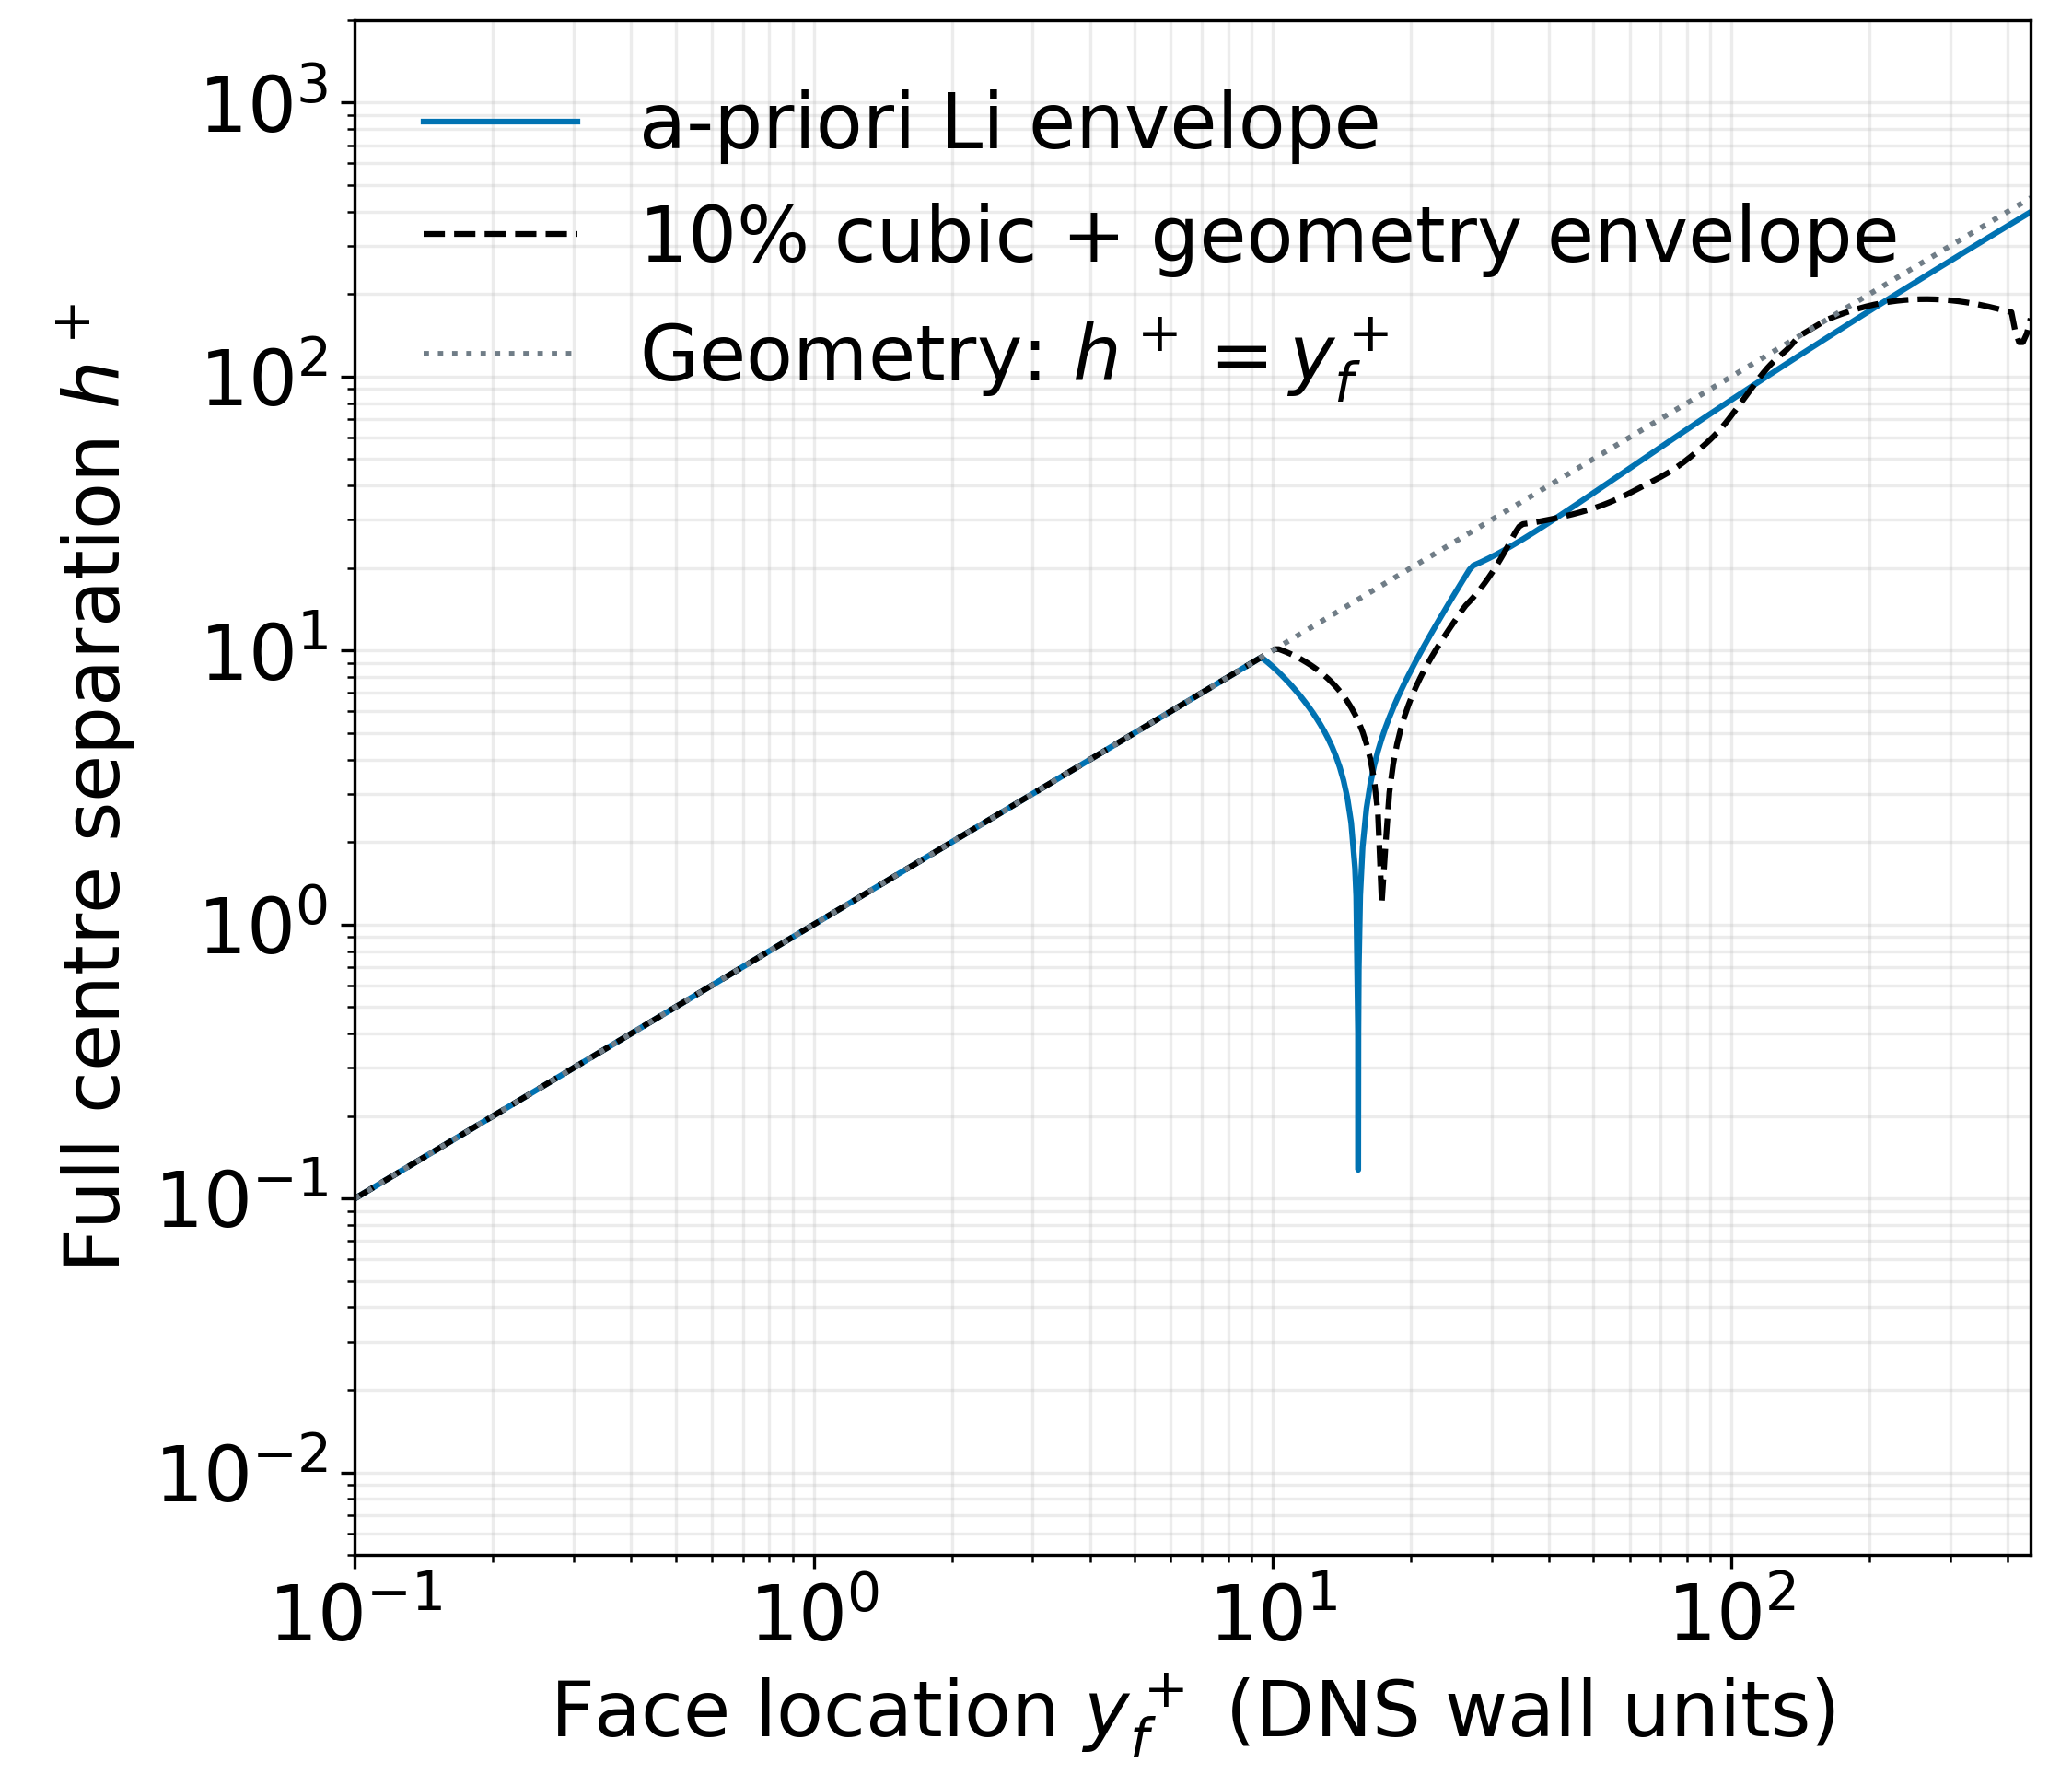
\includegraphics[width=.7\linewidth,height=.54\textheight,keepaspectratio]{07_Error_Isolation_Results/Figures/WallFunctions/apriori_M6_mesh.png}
    \caption{Conditional a-priori estimate of the M6Tw025 $10\%$ spacing envelope from the Li relations (blue), compared with the profile-based cubic-reference envelope (black dashed). The reconstruction uses scalar wall loads, wall/edge states and transport properties, without the resolved boundary layer profile. The geometric cap is dotted. The displaced restrictive minimum near the temperature maximum limits the estimate's use as an accuracy guarantee.}
    \label{fig:WF:a-priori-M6Tw025-10pct-envelope-combined}
\end{figure}

The estimate can consequently guide an initial mesh design or identify a likely region of refinement. Practical use also requires suitable estimates of wall loads and edge quantities. For the present zero-pressure-gradient flat-plates these inputs are comparatively well defined. The boundary layer edge states can be approximated to the freestream conditions, and for the wall heat-flux and shear stress on zero-pressure-gradient flat-plates analytical approximations like the theory of van Driest are available. Their approximation and the validity of the equilibrium assumptions are however more challenging for complex flows.

\subsection{Recovery of the wall-resolved baseline with fitted closures}
\label{subsec:comparative:zpg:fitted-closure}
 
The remaining question, to close the error isolation loop, is whether the wall-function formulation can recover the wall-resolved solution when both its closure relations and spatial discretization errors are removed. LowH\_M3 provides a suitable diagnostic case because its wall-resolved SA thermal-profile shape agrees comparatively well with DNS, thus also eliviating the implications of the turbulence model. The Li formulation is retained, but its velocity and enthalpy relations are fitted to the wall-resolved SA field of the LowH\_M3 case.
\par\medskip

Lookup tables for the wall function's momentum and enthalpy closures are constructed from the wall-resolved SA boundary layer profiles, using the reference wall shear stress, wall heat-flux and local boundary layer edge velocity and temperature. The tables store the fitted velocity relation and a correction to the Li enthalpy relation. During CFD, the fitted closure relations determine wall shear stress and wall heat-flux from the wall-function sample station's velocity and temperature, while the fitted velocity-law derivative supplies the near-wall constraint on the SA variable $\tilde{\nu}$ (Section~\ref{subsec:wall-functions:gao-li:turbulence-coupling}). The construction therefore requires reference profiles at multiple streamwise stations and the singular published DNS profiles are insufficient.
\par\medskip

Figure~\ref{fig:WF:a-priori-Li-fitted-LowHM3} first checks the fitted closure relations using the same a-priori approach as in Section~\ref{subsec:erriso:apriori-solver}. The recovered heat-flux and shear stress differ from the wall-resolved targets by order $10^{-7}\%$. This near-exact recovery verifies the reference-conditioned inverse construction at the sampled states.

\begin{figure}[H]
    \centering
    % Figure provenance (WSL; absolute paths):
    %   Figure: /home/mgnadlinger/OpenFOAM/mgnadlinger-v2412/src/LiWallFunctions/tests/ReverseSolver/LowH_M3_Duan_Li_fitted/wall_flux_errors_vs_yplus.png
    %   Python scripts:
    %     /home/mgnadlinger/OpenFOAM/mgnadlinger-v2412/src/LiWallFunctions/tests/ReverseSolver/analyze_li_fitted_wall_function_profile_Duan.py
    %     /home/mgnadlinger/OpenFOAM/mgnadlinger-v2412/src/LiWallFunctions/tests/ReverseSolver/build_lowh_m3_fitted_model.py
    %   Data / simulation roots (high-level):
    %     /home/mgnadlinger/OpenFOAM/mgnadlinger-v2412/src/LiWallFunctions/tests/ReverseSolver/LowH_M3_Duan
    %     /home/mgnadlinger/OpenFOAM/mgnadlinger-v2412/src/LiWallFunctions/tests/ReverseSolver/LowH_M3_Duan_Li/constant/LiLowHM3Fit
    %     /home/mgnadlinger/OpenFOAM/mgnadlinger-v2412/src/LiWallFunctions/tests/ReverseSolver/LowH_M3_Duan_Li_fitted
    %     /home/mgnadlinger/Duan_DNS_ZPGFP/Martin_Duan_Part4/SA_Prt0p9/LowH_M3
    %     /home/mgnadlinger/WF_validation/LowH_M3/wall_resolved/SA/LowH_M3
    %     /home/mgnadlinger/WF_validation/LowH_M3/Li_SA
    %   Note: Closure input is the wall-resolved SA profile at time 20000.
    %   Note: Thesis image is resized from the source export. The fitted model uses wall-resolved SA profiles
    %     and Li_SA mesh geometry.
    % End figure provenance.
    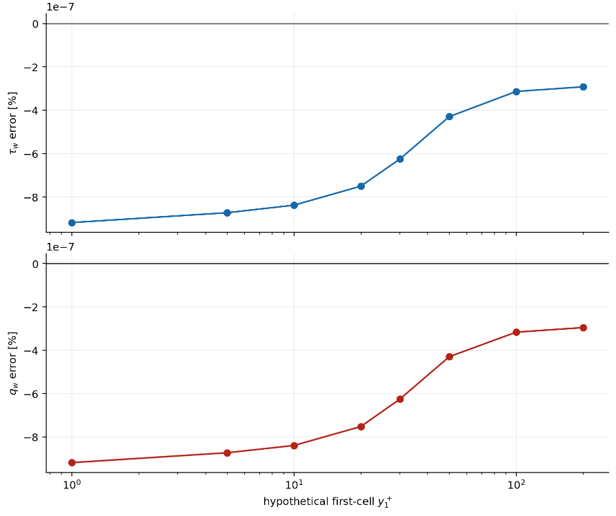
\includegraphics[width=\linewidth,height=.43\textheight,keepaspectratio]{07_Error_Isolation_Results/Figures/WallFunctions/a-priori-Li-fitted-LowHM3.png}
    \caption{A-priori inverse recovery using the fitted LowH\_M3 Li relations and samples from the wall-resolved SA reference. Recovered shear stress (top) and heat-flux (bottom) are compared with that same reference. Errors are of order $10^{-7}\%$, as indicated by the axis multipliers; this is consistency of the reference-conditioned inverse model, rather than independent DNS validation.}
    \label{fig:WF:a-priori-Li-fitted-LowHM3}
\end{figure}

The corresponding CFD result is shown in Figure~\ref{fig:WF:3pct-Li-fitted-LowHM3}. With the fitted relations and boundary layer-informed meshes, heat-flux and shear stress remain within approximately $\pm2\%$ of the wall-resolved values over the completed sampling sweep. Thus successfully isolating the errors caused by spatial discretization and wall-function closure theories. The last persistent error to the DNS reference, is the baseline error of the underlying wall-resolved RANS as discovered in the first Section~\ref{subsec:comparative:zpg:wr-wall-fluxes}. So it can be concluded, that with a boundary layer-informed mesh, improved closure relations and improved RANS turbulence modelling, the wall-function CFD could recover perfect wall heat-flux and shear stress.

\begin{figure}[H]
    \centering
    % Figure provenance (WSL; absolute paths):
    %   Figure: /home/mgnadlinger/WF_validation/LowH_M3/mesh_archives/20260908_before_leading_edge_refinement/Li_fitted_3pct_minCells_SA/results_analysis/wall_flux_sweep/plots/li_fitted_3pct_mincells_sa_dns_station_relative_error.png
    %   Python scripts:
    %     /home/mgnadlinger/WF_validation/LowH_M3/mesh_archives/20260908_before_leading_edge_refinement/Li_fitted_3pct_minCells_SA/results_analysis/run_wall_flux_sweep.py
    %     /home/mgnadlinger/WF_validation/LowH_M3/validation/scripts/plot_wall_flux_sweeps.py
    %   Data / simulation roots (high-level):
    %     /home/mgnadlinger/WF_validation/LowH_M3/mesh_archives/20260908_before_leading_edge_refinement/Li_fitted_3pct_minCells_SA
    %     /home/mgnadlinger/WF_validation/LowH_M3/wall_resolved/SA/LowH_M3
    %     /home/mgnadlinger/WF_validation/LowH_M3/Digitizations
    %   Note: Thesis image removes the 128-pixel title strip from the source export.
    %   Note: Displayed CFD results use the archived sweep from before the leading-edge mesh refinement on
    %     2026-09-08.
    %   Note: An identical full export is also retained at
    %     /home/mgnadlinger/WF_validation/LowH_M3/validation/outputs/plots/li_fitted_3pct_mincells_sa_dns_station_relative_error.png
    % End figure provenance.
    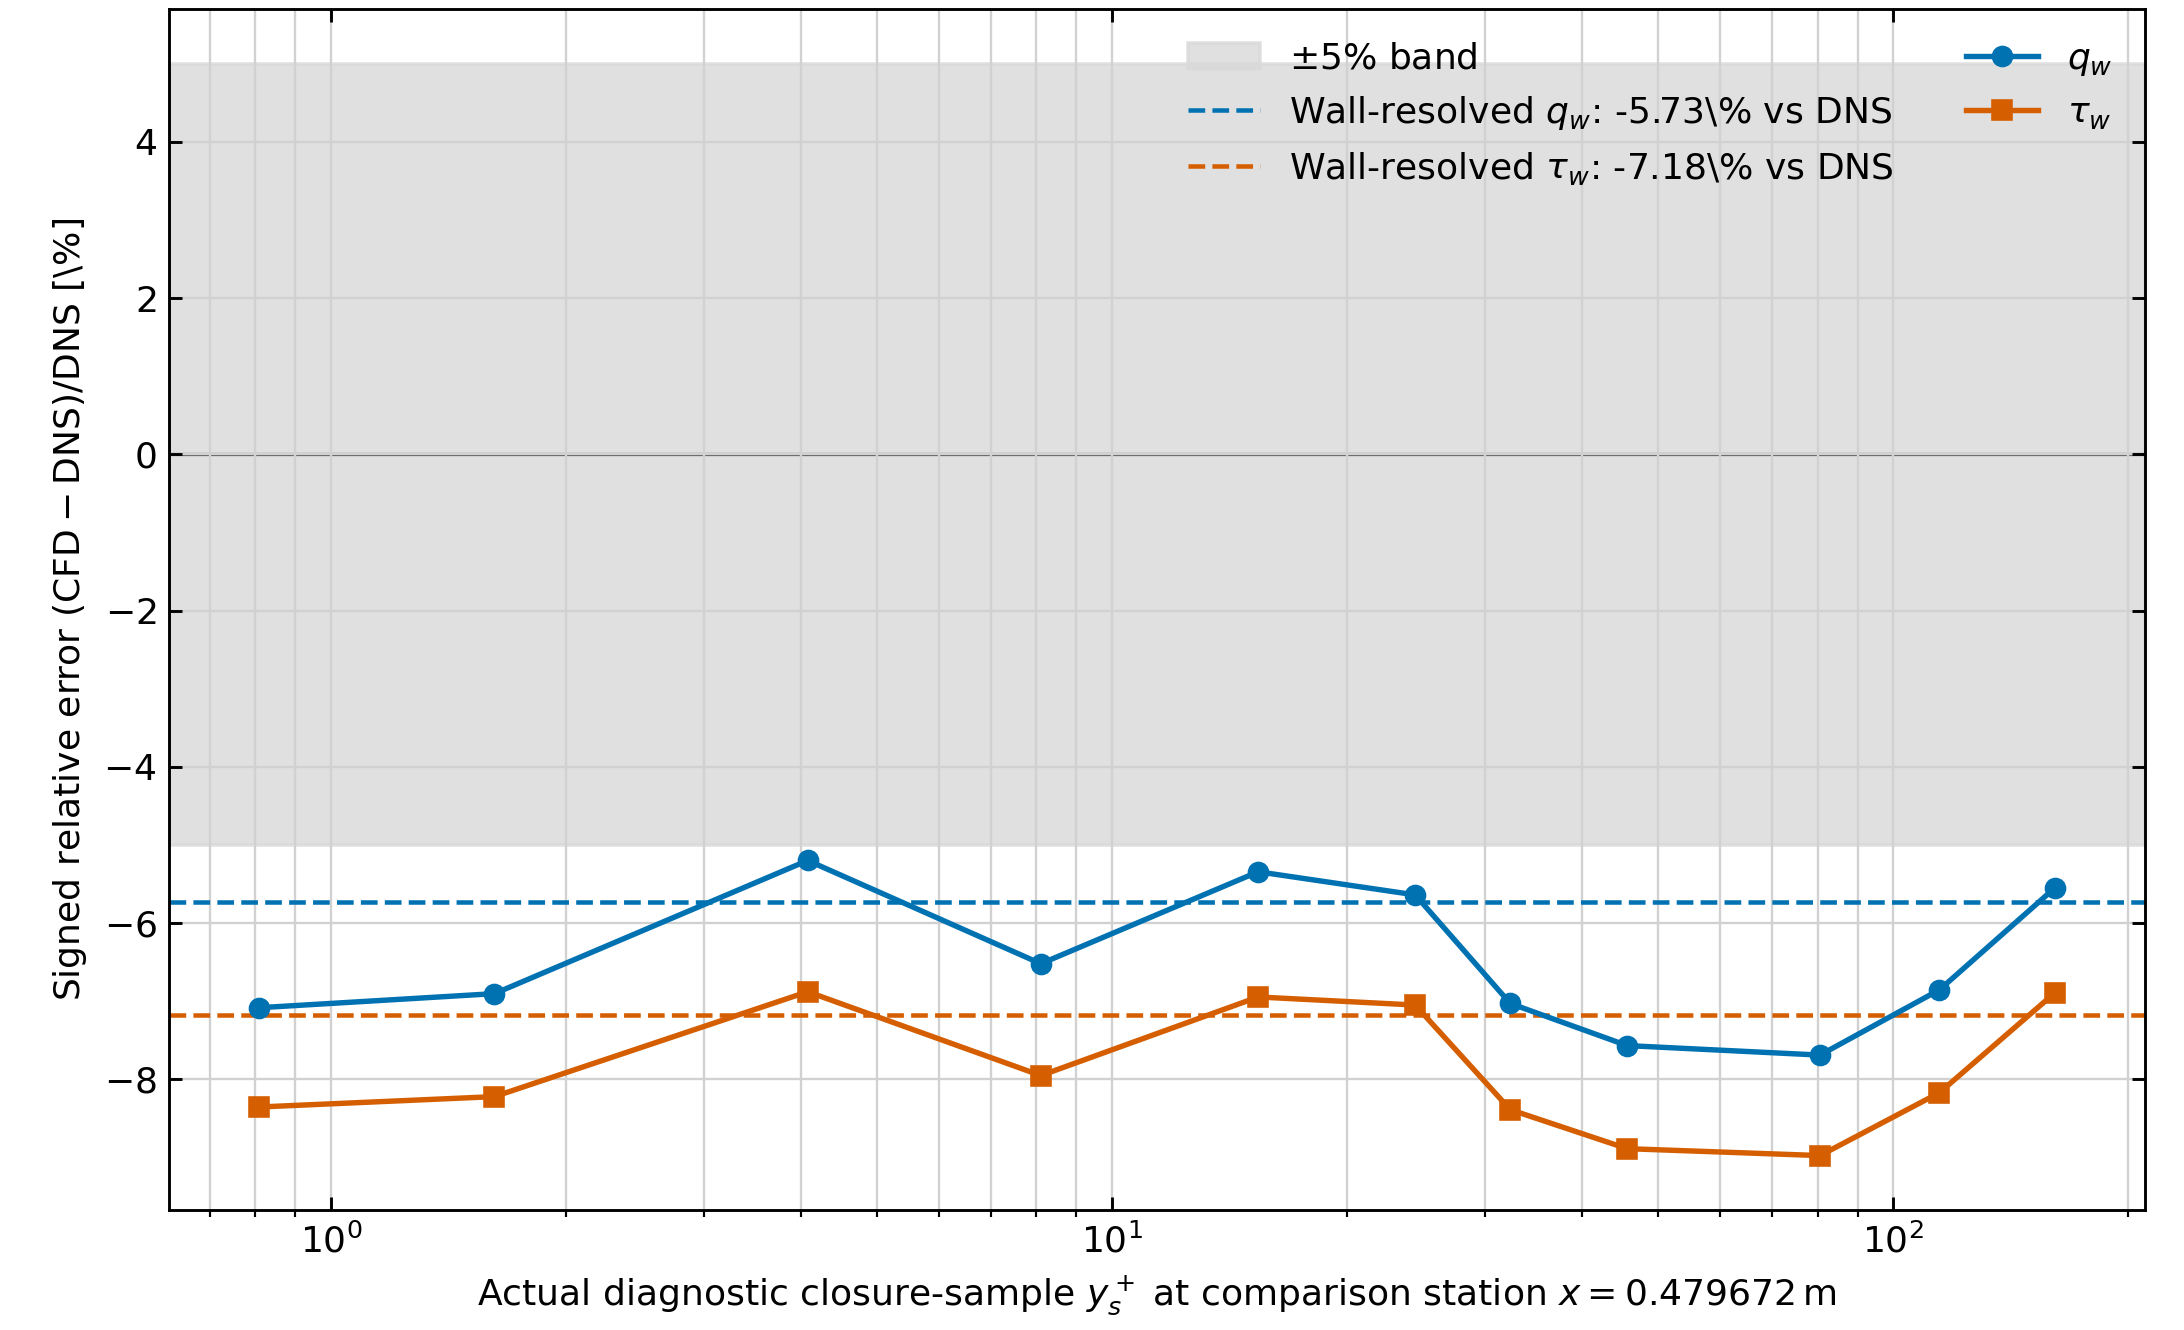
\includegraphics[width=\linewidth,height=.43\textheight,keepaspectratio]{07_Error_Isolation_Results/Figures/WallFunctions/04_3pctMesh_fitted_Li_LowHM3.png}
    \caption{LowH\_M3 CFD with fitted Li relations, SA and boundary layer-informed $3\%$ meshes. Signed errors in heat-flux and shear stress relative to DNS are plotted against the actual sampling location at $x=0.479672\,\mathrm{m}$. The curves remain close to the wall-resolved baseline (dashed), with deviations of approximately $\pm2\%$ when normalized by the corresponding wall-resolved quantities. Shading marks $\pm5\%$ relative to DNS.}
    \label{fig:WF:3pct-Li-fitted-LowHM3}
\end{figure}
